\documentclass[11pt,a4paper]{article}

% -----------------------------------------------------------------------------
% Packages
% -----------------------------------------------------------------------------
\usepackage[utf8]{inputenc}
\usepackage[T1]{fontenc}
\usepackage{lmodern}
\usepackage{microtype}
\usepackage{amsmath,amssymb,amsthm}
\usepackage{mathtools}
\usepackage{bm}
\usepackage{geometry}
\usepackage{hyperref}
\usepackage{cleveref}
\usepackage{enumitem}
\usepackage{booktabs}
\usepackage{array}
\usepackage{listings}
\usepackage{xcolor}
\usepackage{tikz}
\usetikzlibrary{arrows.meta, positioning, calc, fit, matrix, decorations.pathreplacing, shapes.geometric, backgrounds}
\usepackage{algorithm}
\usepackage{algpseudocode}
\usepackage[most]{tcolorbox}
\usepackage{caption}
\usepackage{float}

\geometry{margin=2.5cm}
\hypersetup{
  colorlinks=true,
  linkcolor=blue!70!black,
  citecolor=green!45!black,
  urlcolor=blue!60!black
}

% -----------------------------------------------------------------------------
% Theorem environments
% -----------------------------------------------------------------------------
\theoremstyle{definition}
\newtheorem{definition}{Definition}[section]
\newtheorem{remark}{Remark}[section]
\newtheorem{example}{Example}[section]
\theoremstyle{plain}
\newtheorem{proposition}{Proposition}[section]
\newtheorem{lemma}{Lemma}[section]

% -----------------------------------------------------------------------------
% Boxes
% -----------------------------------------------------------------------------
\newtcolorbox{motivationbox}[1][]{
  colback=green!3!white,
  colframe=green!45!black,
  fonttitle=\bfseries,
  title={#1},
  breakable
}

\newtcolorbox{intuitionbox}[1][]{
  colback=purple!3!white,
  colframe=purple!45!black,
  fonttitle=\bfseries,
  title={#1},
  breakable
}

\newtcolorbox{connectionbox}[1][]{
  colback=cyan!3!white,
  colframe=cyan!55!black,
  fonttitle=\bfseries,
  title={#1},
  breakable
}

\newtcolorbox{tradeoffbox}[1][]{
  colback=red!2!white,
  colframe=red!60!black,
  fonttitle=\bfseries,
  title={#1},
  breakable
}

\newtcolorbox{warningbox}[1][]{
  colback=orange!4!white,
  colframe=orange!70!black,
  fonttitle=\bfseries,
  title={#1},
  breakable
}

% -----------------------------------------------------------------------------
% Code listing style
% -----------------------------------------------------------------------------
\definecolor{codebg}{RGB}{245,245,245}
\definecolor{codeframe}{RGB}{200,200,200}
\lstset{
    language=Python,
    basicstyle=\ttfamily\small,
    backgroundcolor=\color{codebg},
    frame=single,
    rulecolor=\color{codeframe},
    keywordstyle=\color{blue!70!black}\bfseries,
    stringstyle=\color{red!60!black},
    commentstyle=\color{green!50!black}\itshape,
    showstringspaces=false,
    breaklines=true,
    numbers=left,
    numberstyle=\tiny\color{gray},
    xleftmargin=2em,
    framexleftmargin=1.5em,
}

% -----------------------------------------------------------------------------
% Custom commands
% -----------------------------------------------------------------------------
\newcommand{\vx}{\bm{x}}
\newcommand{\vu}{\bm{u}}
\newcommand{\vg}{\bm{g}}
\newcommand{\vq}{\bm{q}}
\newcommand{\vk}{\bm{k}}
\newcommand{\vv}{\bm{v}}
\newcommand{\vo}{\bm{o}}
\newcommand{\vw}{\bm{w}}
\newcommand{\vh}{\bm{h}}
\newcommand{\vy}{\bm{y}}
\newcommand{\vz}{\bm{z}}
\newcommand{\vtheta}{\bm{\theta}}
\newcommand{\mW}{\bm{W}}
\newcommand{\mQ}{\bm{Q}}
\newcommand{\mK}{\bm{K}}
\newcommand{\mV}{\bm{V}}
\newcommand{\mA}{\bm{A}}
\newcommand{\mR}{\bm{R}}
\newcommand{\mI}{\bm{I}}
\newcommand{\mM}{\bm{M}}
\newcommand{\mX}{\bm{X}}
\newcommand{\mY}{\bm{Y}}
\newcommand{\mH}{\bm{H}}
\newcommand{\mO}{\bm{O}}
\newcommand{\mP}{\bm{P}}
\newcommand{\mZ}{\bm{Z}}
\newcommand{\reals}{\mathbb{R}}
\newcommand{\naturals}{\mathbb{N}}
\newcommand{\E}{\mathbb{E}}
\newcommand{\Prob}{\mathbb{P}}
\newcommand{\Var}{\mathrm{Var}}
\newcommand{\Cov}{\mathrm{Cov}}
\newcommand{\dmodel}{d_{\mathrm{model}}}
\newcommand{\dhead}{d_{\mathrm{head}}}
\newcommand{\dff}{d_{\mathrm{ff}}}
\newcommand{\nhead}{n_{\mathrm{head}}}
\newcommand{\nlayer}{n_{\mathrm{layer}}}
\newcommand{\vocab}{|\mathcal{V}|}
\newcommand{\loss}{\mathcal{L}}
\newcommand{\data}{\mathcal{D}}
\newcommand{\ind}{\mathbf{1}}
\newcommand{\given}{\,|\,}
\DeclareMathOperator{\softmax}{softmax}
\DeclareMathOperator{\ReLU}{ReLU}
\DeclareMathOperator{\GELU}{GELU}
\DeclareMathOperator{\SiLU}{SiLU}
\DeclareMathOperator{\RMS}{RMS}
\DeclareMathOperator{\diag}{diag}
\DeclareMathOperator{\KL}{KL}
\DeclareMathOperator{\CE}{CE}
\DeclareMathOperator{\argmax}{arg\,max}

% -----------------------------------------------------------------------------
% TikZ styles
% -----------------------------------------------------------------------------
\tikzset{
  block/.style={draw, rounded corners, thick, align=center, minimum height=8mm, minimum width=22mm, fill=blue!6},
  data/.style={draw, rounded corners, thick, align=center, minimum height=7mm, minimum width=18mm, fill=green!7},
  tensor/.style={draw, rounded corners, thick, align=center, fill=purple!7, minimum height=7mm},
  op/.style={draw, circle, thick, inner sep=1.2pt, fill=white},
  smallblock/.style={draw, rounded corners, thick, align=center, font=\small, fill=blue!5, minimum height=6mm},
  pressure/.style={draw, rounded corners, thick, align=center, fill=orange!8, minimum height=7mm},
  replacement/.style={draw, rounded corners, thick, align=center, fill=green!8, minimum height=7mm},
  arrow/.style={-{Latex[length=2mm]}, thick},
  residual/.style={-{Latex[length=2.3mm]}, very thick, blue!70!black},
  grad/.style={-{Latex[length=2.3mm]}, very thick, red!70!black, dashed},
  note/.style={align=center, font=\small},
  every node/.style={font=\small}
}

% -----------------------------------------------------------------------------
% Title
% -----------------------------------------------------------------------------
\title{\textbf{Transformer Variant Lab: Explained, Motivation-First, and Deduplicated Notes}\\[0.5em]
\large Decoder-Only Transformers from GPT-2 Style V0 to LLaMA-Style V1: Examples, Motivations, and Future-Variant Slots}
\author{Project Notes -- Mathematical Statistics and Machine Learning Level}
\date{\today}

\begin{document}
\maketitle
\tableofcontents
\newpage

% =============================================================================
\section{Introduction and Organization}
% =============================================================================

This document explains two decoder-only Transformer variants implemented in the project. It keeps the important topics from the original notes, but each topic has one home section: definitions, motivations, examples, implementation notes, and trade-offs are placed together rather than repeated in multiple places:
\begin{itemize}
    \item \textbf{V0 (Vanilla):} a GPT-2-style decoder-only Transformer with learned absolute position embeddings, LayerNorm, standard multi-head self-attention, and a ReLU or GELU feed-forward network.
    \item \textbf{V1 (Modern):} a LLaMA-style decoder-only Transformer using Rotary Position Embeddings (RoPE), RMSNorm, SwiGLU feed-forward layers, and FlashAttention-style scaled dot-product attention kernels.
\end{itemize}

The goal is to explain the \emph{reasoning chain} behind the architectural shifts, not merely to list them. The notes therefore use the same pattern inside each component family:
\begin{equation*}
    \text{baseline role}
    \rightarrow
    \text{limitation}
    \rightarrow
    \text{design pressure}
    \rightarrow
    \text{replacement mechanism}
    \rightarrow
    \text{new trade-off}.
\end{equation*}

\begin{motivationbox}[One topic, one home section]
A previous draft repeated the same explanations in a component-shift section, a technical section, and a final roadmap. This version removes that redundancy. Each major topic is discussed in exactly one home section:
\begin{itemize}[nosep]
    \item residual stream and block equations: \cref{sec:block-residual};
    \item statistical objective: \cref{sec:statistical-objective};
    \item normalization and residual stability: \cref{sec:normalization};
    \item attention, positions, RoPE, and FlashAttention: \cref{sec:attention-position};
    \item ReLU/GELU/SiLU and SwiGLU: \cref{sec:ffn};
    \item KV-cache and decoding: \cref{sec:generation};
    \item bias, dropout, and weight tying: \cref{sec:simplifications};
    \item optimization, precision, and evaluation: \cref{sec:training-eval}.
\end{itemize}
Later sections may refer back to these topics, but they do not re-explain them.
\end{motivationbox}

\subsection{Notation}

Throughout, we use the following conventions:
\begin{itemize}[nosep]
    \item $B$ is batch size, $T$ is sequence length, and $\dmodel$ is the residual-stream width.
    \item $\nhead$ is the number of attention heads, and $\dhead=\dmodel/\nhead$ is the dimension per head.
    \item $\dff$ is the standard FFN hidden dimension, and $d_h$ is the SwiGLU hidden dimension.
    \item $\nlayer$ is the number of Transformer blocks.
    \item $\mathcal{V}$ is the vocabulary, and $\vocab$ is its size.
    \item Bold lowercase symbols such as $\vx,\vq,\vk$ denote vectors. Bold uppercase symbols such as $\mW,\mQ,\mK$ denote matrices or tensors.
    \item $\odot$ denotes element-wise multiplication, and $\sigma(x)=(1+e^{-x})^{-1}$ is the logistic sigmoid.
\end{itemize}

\subsection{Tensor-shape conventions}

For a mini-batch of token IDs $\bm{s}\in\{1,\ldots,\vocab\}^{B\times T}$, the embedding layer returns
\begin{equation}
    \mX^{(0)}\in\reals^{B\times T\times \dmodel}.
\end{equation}
For attention, query, key, and value tensors are usually reshaped to
\begin{equation}
    \mQ,\mK,\mV\in\reals^{B\times\nhead\times T\times\dhead}.
\end{equation}
The final logits have shape
\begin{equation}
    \mZ\in\reals^{B\times T\times\vocab}.
\end{equation}
Keeping shapes explicit prevents many implementation mistakes, especially when adding RoPE or a KV-cache.

% =============================================================================
\section{Statistical Objective}
\label{sec:statistical-objective}
% =============================================================================

\subsection{Autoregressive factorization}

A decoder-only language model defines a probability distribution over token sequences $s_{1:T}$ by the chain rule:
\begin{equation}\label{eq:chain_rule_lm}
    p_{\vtheta}(s_{1:T})=
    \prod_{t=1}^{T}p_{\vtheta}(s_t\given s_{<t}),
\end{equation}
where $s_{<t}=(s_1,\ldots,s_{t-1})$ and $\vtheta$ denotes all trainable parameters. Causal masking is the architectural enforcement of this conditioning restriction: the prediction at position $t$ must not use tokens $s_{t+1},\ldots,s_T$.

\begin{figure}[H]
\centering
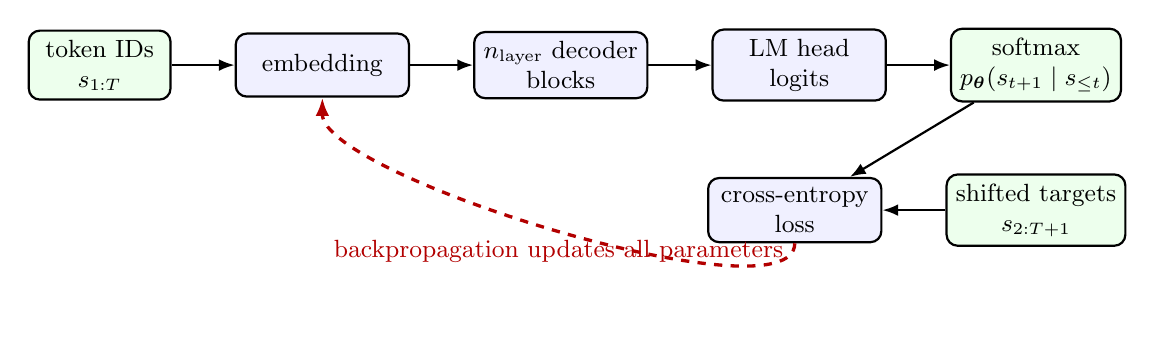
\begin{tikzpicture}[node distance=9mm and 8mm]
    \node[data] (tokens) {token IDs\\$s_{1:T}$};
    \node[block, right=of tokens] (emb) {embedding};
    \node[block, right=of emb] (blocks) {$\nlayer$ decoder\\blocks};
    \node[block, right=of blocks] (head) {LM head\\logits};
    \node[data, right=of head] (prob) {softmax\\$p_{\vtheta}(s_{t+1}\mid s_{\le t})$};
    \node[data, below=9mm of prob] (target) {shifted targets\\$s_{2:T+1}$};
    \node[block, left=of target] (loss) {cross-entropy\\loss};

    \draw[arrow] (tokens) -- (emb);
    \draw[arrow] (emb) -- (blocks);
    \draw[arrow] (blocks) -- (head);
    \draw[arrow] (head) -- (prob);
    \draw[arrow] (prob) -- (loss);
    \draw[arrow] (target) -- (loss);
    \draw[grad] (loss.south) .. controls +(0,-1.0) and +(0,-1.0) .. node[below, note] {backpropagation updates all parameters} (emb.south);
\end{tikzpicture}
\caption{Training flow for a decoder-only language model. V0 and V1 change the internal parameterization of the decoder blocks, but the objective remains shifted-token maximum likelihood.}
\label{fig:training-flow}
\end{figure}

Given a dataset $\data=\{s^{(i)}_{1:T_i}\}_{i=1}^N$, maximum likelihood estimation minimizes the negative log-likelihood:
\begin{equation}\label{eq:nll}
    \loss(\vtheta)=
    -\sum_{i=1}^{N}\sum_{t=1}^{T_i}
    \log p_{\vtheta}\!\left(s^{(i)}_t\given s^{(i)}_{<t}\right).
\end{equation}
The average token-level loss is
\begin{equation}\label{eq:avg_nll}
    \bar{\loss}(\vtheta)=
    -\frac{1}{M}\sum_{i=1}^{N}\sum_{t=1}^{T_i}
    \log p_{\vtheta}\!\left(s^{(i)}_t\given s^{(i)}_{<t}\right),
    \qquad M=\sum_{i=1}^{N}T_i.
\end{equation}

\subsection{Cross-entropy and KL divergence}

Let $q$ be the true conditional next-token distribution and $p_{\vtheta}$ the model distribution. For a fixed context,
\begin{equation}\label{eq:cross_entropy_def}
    H(q,p_{\vtheta})
    =-\sum_{w\in\mathcal{V}}q(w)\log p_{\vtheta}(w).
\end{equation}
The KL decomposition is
\begin{equation}\label{eq:entropy_decomposition}
    H(q,p_{\vtheta})=H(q)+\KL(q\Vert p_{\vtheta}).
\end{equation}
Since $H(q)$ does not depend on $\vtheta$, minimizing cross-entropy is equivalent, at the population level, to minimizing $\KL(q\Vert p_{\vtheta})$.

In data, we observe one true next token per context. The empirical target is a one-hot distribution
\begin{equation}
    \hat q(w)=\ind[w=s^{\mathrm{true}}_t],
\end{equation}
so the cross-entropy collapses to
\begin{equation}
    H(\hat q,p_{\vtheta})=-\log p_{\vtheta}(s^{\mathrm{true}}_t\given s_{<t}).
\end{equation}
This is the per-token training loss used in code.

\begin{motivationbox}[Why the statistical objective matters]
The architecture is not directly trained to ``sound good.'' It is trained to assign high probability to the next token under held-out contexts. A component is useful if it lowers validation cross-entropy, reaches the same loss faster, or computes the same probability distribution with less memory and time.
\end{motivationbox}

\subsection{Perplexity}

Perplexity is the exponential of the average NLL:
\begin{equation}\label{eq:perplexity}
    \mathrm{PPL}=\exp(\bar{\loss}).
\end{equation}
If the average loss is measured in nats, perplexity can be interpreted as an effective branching factor. A perplexity of $20$ means that the model is, on average, about as uncertain as choosing uniformly among $20$ plausible next tokens. This interpretation is approximate because real next-token distributions are not uniform.

\subsection{Empirical risk, validation loss, and tokenization}

Training loss is an empirical estimate of population risk. A separate validation set estimates out-of-sample risk:
\begin{equation}
    \widehat R_{\mathrm{val}}(\vtheta)=
    -\frac{1}{M_{\mathrm{val}}}\sum_{(i,t)\in\mathrm{val}}
    \log p_{\vtheta}(s^{(i)}_t\given s^{(i)}_{<t}).
\end{equation}
The generalization gap is
\begin{equation}
    \widehat R_{\mathrm{val}}(\vtheta)-\widehat R_{\mathrm{train}}(\vtheta).
\end{equation}
A small model can underfit, giving high training and validation loss. A large model trained too long on too little data can overfit, giving low training loss but worse validation loss.

The model distribution is over tokens, not directly over words or characters. Therefore, perplexities are only comparable when the tokenizer, vocabulary, data split, and context length are held fixed.

\begin{warningbox}[Data leakage]
Validation loss is meaningful only if validation text is not duplicated in the training set. If validation documents leak into training, the validation loss becomes an optimistic estimate of generalization.
\end{warningbox}

% =============================================================================
\section{Decoder Block and Residual Stream}
\label{sec:block-residual}
% =============================================================================

\subsection{Input representation}

In V0, the initial residual stream is the sum of token and learned position embeddings:
\begin{equation}\label{eq:v0_embedding}
    \mX^{(0)}_{b,t,:}=\mW_{\mathrm{tok}}[s_{b,t}]+\mW_{\mathrm{pos}}[t].
\end{equation}
In V1, RoPE is applied inside attention, so the initial residual stream uses token embeddings only:
\begin{equation}\label{eq:v1_embedding}
    \mX^{(0)}_{b,t,:}=\mW_{\mathrm{tok}}[s_{b,t}].
\end{equation}

\subsection{Residual stream}

\begin{definition}[Residual stream]
The \emph{residual stream} is the hidden representation of all tokens as it flows through the Transformer:
\begin{equation}
    \mX^{(0)},\mX^{(1)},\ldots,\mX^{(\nlayer)}
    \in\reals^{B\times T\times\dmodel}.
\end{equation}
Each block updates this stream additively:
\begin{equation}
    \mX\leftarrow\mX+\mathrm{Sublayer}(\mathrm{Norm}(\mX)).
\end{equation}
Thus, the residual stream is not a separate parameter matrix. It is the evolving token representation that attention and FFN sublayers repeatedly read from and write to.
\end{definition}

Attention writes cross-token information into the residual stream. The FFN writes nonlinear token-wise features into the same stream. This is why architecture choices interact: if the FFN update becomes stronger, normalization and initialization must still keep the additive stream stable.

\begin{figure}[H]
\centering
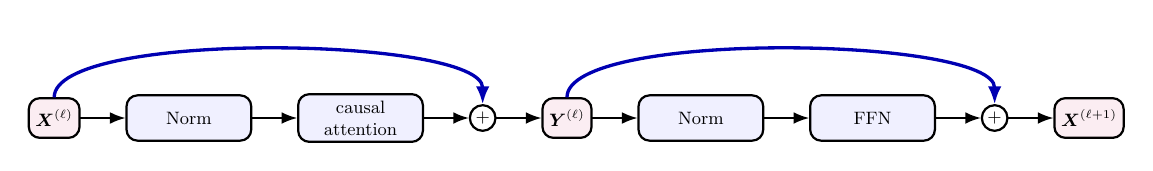
\begin{tikzpicture}[scale=0.72, transform shape, node distance=7mm and 8mm]
    \node[tensor] (x) {$\mX^{(\ell)}$};
    \node[block, right=of x] (n1) {Norm};
    \node[block, right=of n1] (attn) {causal\\attention};
    \node[op, right=of attn] (p1) {$+$};
    \node[tensor, right=of p1] (y) {$\mY^{(\ell)}$};
    \node[block, right=of y] (n2) {Norm};
    \node[block, right=of n2] (ffn) {FFN};
    \node[op, right=of ffn] (p2) {$+$};
    \node[tensor, right=of p2] (out) {$\mX^{(\ell+1)}$};

    \draw[arrow] (x) -- (n1);
    \draw[arrow] (n1) -- (attn);
    \draw[arrow] (attn) -- (p1);
    \draw[arrow] (p1) -- (y);
    \draw[arrow] (y) -- (n2);
    \draw[arrow] (n2) -- (ffn);
    \draw[arrow] (ffn) -- (p2);
    \draw[arrow] (p2) -- (out);
    \draw[residual] (x.north) .. controls +(0,1.2) and +(0,1.2) .. (p1.north);
    \draw[residual] (y.north) .. controls +(0,1.2) and +(0,1.2) .. (p2.north);
\end{tikzpicture}
\caption{Pre-normalized residual block. Normalization controls the input scale of each sublayer; residual arrows preserve a direct information and gradient path.}
\label{fig:preln-block}
\end{figure}

\subsection{Block equations}

For layer $\ell=0,\ldots,\nlayer-1$:
\begin{align}
    \mY^{(\ell)}
    &=\mX^{(\ell)}+
      \mathrm{Attn}^{(\ell)}\!\left(\mathrm{Norm}^{(\ell)}_1(\mX^{(\ell)})\right),\label{eq:block_attn}\\
    \mX^{(\ell+1)}
    &=\mY^{(\ell)}+
      \mathrm{FFN}^{(\ell)}\!\left(\mathrm{Norm}^{(\ell)}_2(\mY^{(\ell)})\right).\label{eq:block_ffn}
\end{align}
A final normalization is often applied before the output head:
\begin{equation}\label{eq:final_norm_logits}
    \mH=\mathrm{Norm}_{\mathrm{final}}(\mX^{(\nlayer)}),
    \qquad
    \mZ=\mH\mW_{\mathrm{head}}^{\top}.
\end{equation}
The conditional probability is
\begin{equation}\label{eq:lm_softmax}
    p_{\vtheta}(s_{t+1}=w\given s_{\le t})=
    \frac{\exp(Z_{t,w})}{\sum_{u\in\mathcal{V}}\exp(Z_{t,u})}.
\end{equation}

\subsection{Stable softmax}

For numerical stability, softmax is computed after subtracting the row maximum:
\begin{equation}\label{eq:stable_softmax}
    \softmax(\vz)_i=
    \frac{\exp(z_i-c)}{\sum_j\exp(z_j-c)},
    \qquad c=\max_j z_j.
\end{equation}
This does not change the mathematical value because softmax is shift-invariant:
\begin{equation}
    \softmax(\vz+c\mathbf{1})=\softmax(\vz).
\end{equation}
It prevents overflow when logits are large.

\subsection{Parameter-count accounting}

A rough parameter count is useful when comparing variants.
\begin{itemize}[nosep]
    \item \textbf{Embeddings:} token embeddings contain $\vocab\dmodel$ parameters. Learned absolute position embeddings add $T_{\max}\dmodel$ parameters in V0. RoPE adds no trainable parameters in V1.
    \item \textbf{Attention:} standard dense Q, K, V, and output projections contain approximately $4\dmodel^2$ parameters per layer, ignoring biases.
    \item \textbf{Standard FFN:} a two-matrix FFN with $\dff=4\dmodel$ contains $2\dmodel\dff=8\dmodel^2$ parameters per layer.
    \item \textbf{SwiGLU FFN:} a gated FFN with hidden size $d_h$ contains $3\dmodel d_h$ parameters. Parameter matching with the standard FFN gives $d_h\approx(8/3)\dmodel$.
\end{itemize}
Ignoring normalization scales, a decoder layer therefore has about $4\dmodel^2+8\dmodel^2=12\dmodel^2$ non-embedding parameters when the FFN is parameter-matched.

% =============================================================================
\section{Residual Stability and Normalization}
\label{sec:normalization}
% =============================================================================

\subsection{The scaling problem created by residual additions}

A residual block adds a learned update to its input:
\begin{equation}\label{eq:residual}
    \vx^{(\ell+1)}=\vx^{(\ell)}+f^{(\ell)}(\vx^{(\ell)}).
\end{equation}
If residual updates were independent and had coordinate variance $\sigma_f^2$, then after $L$ additions,
\begin{equation}
    \Var[x_i^{(L)}]\approx \Var[x_i^{(0)}]+L\sigma_f^2.
\end{equation}
The independence assumption is only a heuristic, but it shows the risk: residual streams can drift in scale with depth. Normalization and initialization address this problem from opposite sides. Normalization controls the input scale to each sublayer; residual-output initialization controls the update scale written back into the stream.

\subsection{Pre-normalization versus post-normalization}

The original Transformer used post-normalization:
\begin{equation}
    \vx^{(\ell+1)}=\mathrm{Norm}\bigl(\vx^{(\ell)}+f^{(\ell)}(\vx^{(\ell)})\bigr).
\end{equation}
Modern decoder-only language models usually use pre-normalization:
\begin{equation}\label{eq:preln}
    \vx^{(\ell+1)}=\vx^{(\ell)}+f^{(\ell)}(\mathrm{Norm}(\vx^{(\ell)})).
\end{equation}

\begin{proposition}[Direct gradient path in Pre-LN]
For \cref{eq:preln}, the layer Jacobian is
\begin{equation}
    \frac{\partial\vx^{(\ell+1)}}{\partial\vx^{(\ell)}}
    =\mI+J_{f^{(\ell)}}J_{\mathrm{Norm}}.
\end{equation}
The identity term gives a direct residual path for forward activations and backward gradients.
\end{proposition}

\begin{proof}
Differentiate $\vx^{(\ell)}+f^{(\ell)}(\mathrm{Norm}(\vx^{(\ell)}))$ with respect to $\vx^{(\ell)}$ and apply the chain rule.
\end{proof}

This does not guarantee perfect gradient behavior, because products of matrices $\mI+J_fJ_{\mathrm{Norm}}$ can still become poorly conditioned. It does, however, make deep optimization easier than putting normalization directly on the residual path.

\subsection{Component shift: LayerNorm to RMSNorm}

\subsubsection{Baseline role: LayerNorm}

\begin{definition}[Layer Normalization]
For $\vx\in\reals^d$,
\begin{equation}\label{eq:layernorm}
    \mathrm{LayerNorm}(\vx)
    =\bm{\gamma}\odot\frac{\vx-\mu\mathbf{1}}{\sqrt{\sigma^2+\epsilon}}+\bm{\beta},
\end{equation}
where
\begin{equation}
    \mu=\frac{1}{d}\sum_{i=1}^{d}x_i,
    \qquad
    \sigma^2=\frac{1}{d}\sum_{i=1}^{d}(x_i-\mu)^2.
\end{equation}
\end{definition}

LayerNorm performs two operations: it subtracts the feature mean and divides by the feature standard deviation. In V0, this gives each attention and FFN sublayer inputs with predictable coordinate scale.

\subsubsection{Limitation and design pressure}

LayerNorm couples two ideas: re-centering and re-scaling. Re-scaling is directly tied to residual-stream stability: if the input norm doubles, attention logits and FFN activations can become much larger. Re-centering is less obviously essential in pre-normalized decoder-only models, because later linear maps and residual additions can already represent shifted directions. It also adds another reduction over the hidden dimension.

The design pressure is therefore: keep the scale-control part of normalization, simplify the computation, and preserve the pre-norm residual highway.

\subsubsection{Replacement mechanism: RMSNorm}

\begin{definition}[Root Mean Square Normalization]
For $\vx\in\reals^d$,
\begin{equation}\label{eq:rmsnorm}
    \mathrm{RMSNorm}(\vx)=
    \bm{\gamma}\odot\frac{\vx}{\RMS(\vx)},
    \qquad
    \RMS(\vx)=\sqrt{\frac{1}{d}\sum_{i=1}^{d}x_i^2+\epsilon}.
\end{equation}
\end{definition}

RMSNorm removes mean-centering and preserves scale normalization. Since
\begin{equation}\label{eq:rms_variance_relation}
    \RMS(\vx)^2=\frac{1}{d}\Vert\vx\Vert_2^2=\sigma^2+\mu^2,
\end{equation}
RMSNorm is close to LayerNorm when the coordinate mean is small. Unlike LayerNorm, it is not invariant to shifts $\vx\mapsto\vx+c\mathbf{1}$.

\begin{figure}[H]
\centering
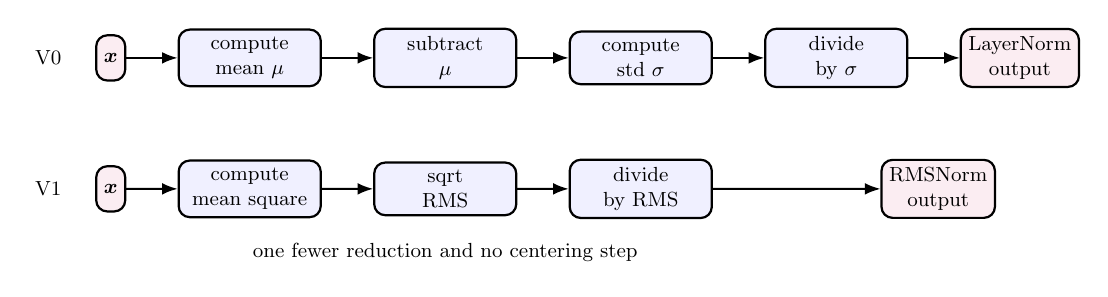
\begin{tikzpicture}[scale=0.82, transform shape, node distance=6mm and 8mm]
    \node[tensor] (x1) {$\vx$};
    \node[block, right=of x1] (mean) {compute\\mean $\mu$};
    \node[block, right=of mean] (center) {subtract\\$\mu$};
    \node[block, right=of center] (std) {compute\\std $\sigma$};
    \node[block, right=of std] (div1) {divide\\by $\sigma$};
    \node[tensor, right=of div1] (ln) {LayerNorm\\output};

    \node[tensor, below=13mm of x1] (x2) {$\vx$};
    \node[block, right=of x2] (ms) {compute\\mean square};
    \node[block, right=of ms] (rms) {sqrt\\RMS};
    \node[block, right=of rms] (div2) {divide\\by RMS};
    \node[tensor, right=26mm of div2] (rn) {RMSNorm\\output};

    \draw[arrow] (x1) -- (mean);
    \draw[arrow] (mean) -- (center);
    \draw[arrow] (center) -- (std);
    \draw[arrow] (std) -- (div1);
    \draw[arrow] (div1) -- (ln);

    \draw[arrow] (x2) -- (ms);
    \draw[arrow] (ms) -- (rms);
    \draw[arrow] (rms) -- (div2);
    \draw[arrow] (div2) -- (rn);

    \node[note, left=4mm of x1] {V0};
    \node[note, left=4mm of x2] {V1};
    \node[note, below=3mm of rms] {one fewer reduction and no centering step};
\end{tikzpicture}
\caption{LayerNorm versus RMSNorm. RMSNorm keeps scale control but drops explicit mean-centering.}
\label{fig:ln-vs-rms}
\end{figure}

\subsubsection{New trade-off and connections}

RMSNorm is not simply a better LayerNorm. It gives up exact shift invariance. If a large common offset across coordinates becomes harmful, RMSNorm will not remove it. The reason it works well in this design is that pre-normalization mostly needs stable magnitudes before sublayers read from the residual stream.

\begin{connectionbox}[Where the connection belongs]
The main connection is local to this section: RMSNorm controls the input scale to attention and FFN sublayers. Later sections mention this only as a cross-reference. For example, SwiGLU is scale-sensitive because it multiplies two projections, but the detailed explanation of RMSNorm remains here.
\end{connectionbox}

\subsection{RMSNorm Jacobian}

Let
\begin{equation}
    r(\vx)=\sqrt{\frac{1}{d}\Vert\vx\Vert_2^2+\epsilon},
    \qquad
    \vy=\frac{\vx}{r(\vx)}.
\end{equation}
Ignoring the learned scale $\bm{\gamma}$, the Jacobian is
\begin{equation}\label{eq:rms_jacobian}
    \frac{\partial\vy}{\partial\vx}
    =\frac{1}{r}\mI-\frac{1}{d r^3}\vx\vx^\top.
\end{equation}
Thus RMSNorm is not merely division by a constant; it couples coordinates through a rank-one correction.

\subsection{Weight initialization and residual-output initialization}

Initialization is part of the architecture story because the model is optimized from its initial function. A deep residual network can be expressive in principle but unstable in practice if every layer initially writes updates that are too large.

For a linear layer $\vy=\mW\vx$ with independent weights and inputs,
\begin{equation}
    \Var(y_i)=d_{\mathrm{in}}\Var(W_{ij})\Var(x_j).
\end{equation}
This is the motivation behind Xavier/Glorot-style initialization: choose weight variance on the order of $1/d_{\mathrm{in}}$ so that activation variance does not systematically grow or shrink after one matrix multiplication.

\begin{intuitionbox}[What initialization controls]
If weights are too small, all features start near zero and gradients can become weak. If weights are too large, activations and attention logits can saturate. Good initialization makes the first forward pass look like a stable random feature model rather than a numerical accident.
\end{intuitionbox}

GPT-2-style models often initialize most weights as
\begin{equation}
    W_{ij}\sim\mathcal{N}(0,0.02^2),
\end{equation}
with a special depth scaling for residual output projections:
\begin{equation}\label{eq:gpt2_init}
    W_{ij}\sim\mathcal{N}\!\left(0,\frac{0.02^2}{2\nlayer}\right)
\end{equation}
for attention output projections and FFN output projections. The factor $2\nlayer$ appears because each block has two residual additions: one from attention and one from the FFN.

\begin{motivationbox}[Why residual projections are scaled more strongly]
The output projection of attention and the down projection of the FFN are the matrices that write into the residual stream. If each of the $2\nlayer$ writes contributes variance of similar size, the total residual variance can grow with depth. Scaling these projections by roughly $1/\sqrt{2\nlayer}$ makes the initial network closer to an identity map plus many small updates.
\end{motivationbox}

\begin{figure}[H]
\centering
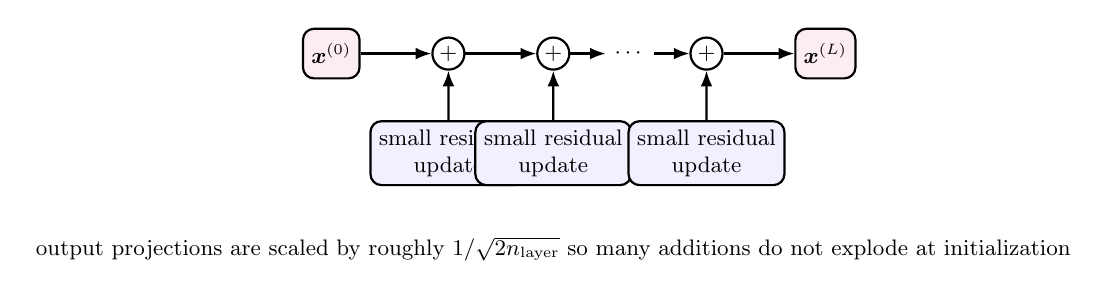
\begin{tikzpicture}[scale=0.90, transform shape, node distance=8mm and 10mm]
    \node[tensor] (x0) {$\vx^{(0)}$};
    \node[op, right=of x0] (p1) {$+$};
    \node[op, right=of p1] (p2) {$+$};
    \node[right=5mm of p2] (dots) {$\cdots$};
    \node[op, right=5mm of dots] (pL) {$+$};
    \node[tensor, right=of pL] (xL) {$\vx^{(L)}$};
    \node[block, below=7mm of p1] (u1) {small residual\\update};
    \node[block, below=7mm of p2] (u2) {small residual\\update};
    \node[block, below=7mm of pL] (uL) {small residual\\update};

    \draw[arrow] (x0) -- (p1);
    \draw[arrow] (p1) -- (p2);
    \draw[arrow] (p2) -- (dots);
    \draw[arrow] (dots) -- (pL);
    \draw[arrow] (pL) -- (xL);
    \draw[arrow] (u1) -- (p1);
    \draw[arrow] (u2) -- (p2);
    \draw[arrow] (uL) -- (pL);
    \node[note, below=6mm of u2] {output projections are scaled by roughly $1/\sqrt{2\nlayer}$ so many additions do not explode at initialization};
\end{tikzpicture}
\caption{Depth-scaled residual projection initialization. The network starts near an identity-plus-small-updates system.}
\label{fig:init-scaling}
\end{figure}

% =============================================================================
\section{Attention, Position, and Attention Computation}
\label{sec:attention-position}
% =============================================================================

\subsection{Self-attention without position is permutation-equivariant}

Without positional information, self-attention is not a sequence model in the usual sense. It is permutation-equivariant: if the input token representations are permuted, the output vectors are permuted in the same way.

\begin{proposition}[Permutation equivariance]
Let $P$ be a permutation matrix applied to the sequence dimension. If no positional information or causal mask is used, then self-attention satisfies
\begin{equation}
    \mathrm{Attn}(P\mX)=P\,\mathrm{Attn}(\mX).
\end{equation}
\end{proposition}
This is why a decoder-only Transformer needs both position information and causal masking.

\subsection{Q, K, and V as content-addressable memory}

\begin{definition}[Scaled dot-product attention]
Given $\mQ\in\reals^{T_q\times\dhead}$, $\mK\in\reals^{T_k\times\dhead}$, and $\mV\in\reals^{T_k\times\dhead}$,
\begin{equation}\label{eq:attention}
    \mathrm{Attention}(\mQ,\mK,\mV)=
    \softmax\!\left(\frac{\mQ\mK^\top}{\sqrt{\dhead}}\right)\mV.
\end{equation}
\end{definition}

Queries and keys decide \emph{where} to read; values contain \emph{what} is read. This separation allows routing and content to use different learned representations.

\begin{figure}[H]
\centering
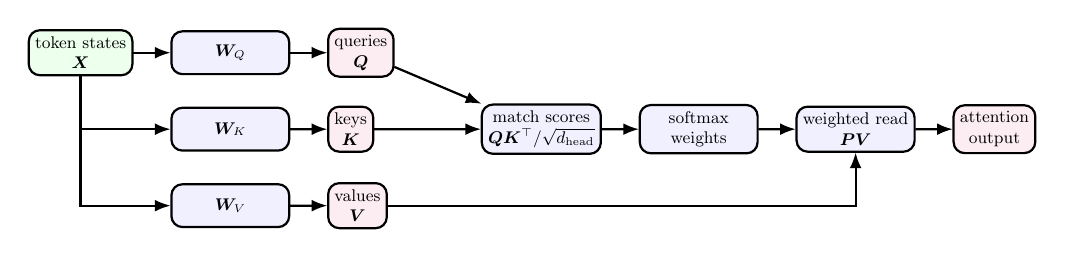
\begin{tikzpicture}[scale=0.68, transform shape, node distance=7mm and 7mm]
    \node[data] (x) {token states\\$\mX$};
    \node[block, right=of x] (wq) {$\mW_Q$};
    \node[tensor, right=of wq] (q) {queries\\$\mQ$};
    \node[block, below=6mm of wq] (wk) {$\mW_K$};
    \node[tensor, right=of wk] (k) {keys\\$\mK$};
    \node[block, below=6mm of wk] (wv) {$\mW_V$};
    \node[tensor, right=of wv] (v) {values\\$\mV$};

    \node[block, right=20mm of k] (score) {match scores\\$\mQ\mK^\top/\sqrt{\dhead}$};
    \node[block, right=of score] (sm) {softmax\\weights};
    \node[block, right=of sm] (read) {weighted read\\$\mP\mV$};
    \node[tensor, right=of read] (out) {attention\\output};

    \draw[arrow] (x) -- (wq);
    \draw[arrow] (x) |- (wk);
    \draw[arrow] (x) |- (wv);
    \draw[arrow] (wq) -- (q);
    \draw[arrow] (wk) -- (k);
    \draw[arrow] (wv) -- (v);
    \draw[arrow] (q) -- (score);
    \draw[arrow] (k) -- (score);
    \draw[arrow] (score) -- (sm);
    \draw[arrow] (sm) -- (read);
    \draw[arrow] (v) -| (read);
    \draw[arrow] (read) -- (out);
\end{tikzpicture}
\caption{Attention as content-addressable memory. Q and K solve the routing problem; V stores the content that is aggregated.}
\label{fig:qkv-memory}
\end{figure}

\subsection{Why divide by \texorpdfstring{$\sqrt{\dhead}$}{sqrt(d-head)}}

Assume $q_i$ and $k_i$ are independent, mean-zero, variance-one random variables. Then
\begin{equation}
    \E[\vq^\top\vk]=0,
    \qquad
    \Var(\vq^\top\vk)=\sum_{i=1}^{\dhead}\Var(q_i k_i)=\dhead.
\end{equation}
Thus the unscaled dot product typically has magnitude $O(\sqrt{\dhead})$. Dividing by $\sqrt{\dhead}$ keeps logits at approximately unit scale and prevents the softmax from saturating at initialization.

\subsection{Causal masking}

For autoregressive language modeling, token $i$ may only attend to tokens $j\leq i$:
\begin{equation}\label{eq:causal_mask}
    A_{ij}=\begin{cases}
        \vq_i^\top\vk_j/\sqrt{\dhead}, & j\leq i,\\
        -\infty, & j>i.
    \end{cases}
\end{equation}
After softmax, entries with $j>i$ receive probability zero.

\begin{figure}[H]
\centering
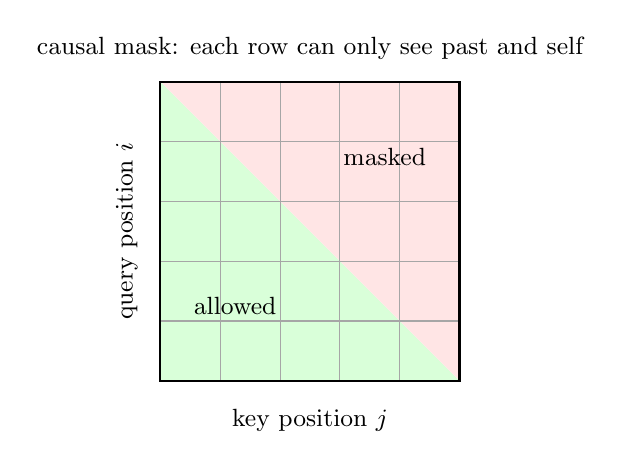
\begin{tikzpicture}[scale=0.95]
    \fill[green!15] (0,0) -- (0,4) -- (4,0) -- cycle;
    \fill[red!10] (0,4) -- (4,4) -- (4,0) -- cycle;
    \draw[step=0.8cm, gray!70] (0,0) grid (4,4);
    \draw[thick] (0,0) rectangle (4,4);
    \node at (1.0,1.0) {allowed};
    \node at (3.0,3.0) {masked};
    \node[below] at (2,-0.25) {key position $j$};
    \node[rotate=90] at (-0.45,2) {query position $i$};
    \node[note] at (2,4.45) {causal mask: each row can only see past and self};
\end{tikzpicture}
\caption{Lower-triangular causal mask. Green entries are visible; red entries are forbidden future context.}
\label{fig:causal-mask}
\end{figure}

\subsection{Multi-head attention}

Each head has its own projections:
\begin{equation}
    \mQ^{(h)}=\mX\mW_Q^{(h)},
    \qquad
    \mK^{(h)}=\mX\mW_K^{(h)},
    \qquad
    \mV^{(h)}=\mX\mW_V^{(h)}.
\end{equation}
Each head computes attention separately, and the outputs are concatenated and projected:
\begin{equation}\label{eq:mha}
    \mathrm{MHA}(\mX)=
    \mathrm{Concat}(\mathrm{head}_1,\ldots,\mathrm{head}_{\nhead})\mW_O.
\end{equation}
Multiple heads let the model learn different retrieval patterns in parallel. The heads are not an ensemble in the statistical sense because they are jointly trained and mixed by $\mW_O$.

\begin{figure}[H]
\centering
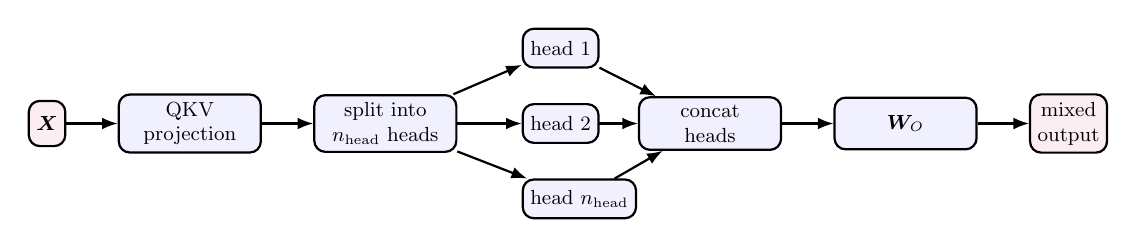
\begin{tikzpicture}[scale=0.82, transform shape, node distance=7mm and 8mm]
    \node[tensor] (x) {$\mX$};
    \node[block, right=of x] (proj) {QKV\\projection};
    \node[block, right=of proj] (split) {split into\\$\nhead$ heads};
    \node[smallblock, above right=4mm and 10mm of split] (h1) {head 1};
    \node[smallblock, right=10mm of split] (h2) {head 2};
    \node[smallblock, below right=4mm and 10mm of split] (h3) {head $\nhead$};
    \node[block, right=28mm of split] (concat) {concat\\heads};
    \node[block, right=of concat] (wo) {$\mW_O$};
    \node[tensor, right=of wo] (out) {mixed\\output};

    \draw[arrow] (x) -- (proj);
    \draw[arrow] (proj) -- (split);
    \draw[arrow] (split) -- (h1);
    \draw[arrow] (split) -- (h2);
    \draw[arrow] (split) -- (h3);
    \draw[arrow] (h1) -- (concat);
    \draw[arrow] (h2) -- (concat);
    \draw[arrow] (h3) -- (concat);
    \draw[arrow] (concat) -- (wo);
    \draw[arrow] (wo) -- (out);
\end{tikzpicture}
\caption{Multi-head attention. Heads learn different retrieval patterns and the output projection writes the mixed result back into the residual stream.}
\label{fig:multihead}
\end{figure}

\subsection{Component shift: learned absolute positions to RoPE}

\subsubsection{Baseline role: learned absolute positions}

V0 injects position by adding a learned lookup-table vector to the token embedding:
\begin{equation}
    \vx_t=\mW_{\mathrm{tok}}[s_t]+\mW_{\mathrm{pos}}[t].
\end{equation}
This is simple and effective, but it treats position as an absolute index. The model learns a vector for ``position 57'' rather than a mechanism for ``three tokens before the current token.'' It is also tied to the maximum number of rows in the learned table.

\subsubsection{Design pressure}

Many language patterns are relative: nearby modifiers, matching brackets, indentation, repeated phrases, and earlier references usually depend on offsets or local structure, not absolute sequence indices. Longer contexts add a second pressure: the position mechanism should extend deterministically beyond a fixed embedding table, even if extrapolation quality is not guaranteed.

\subsubsection{Replacement mechanism: RoPE}

RoPE moves positional information from the input embedding sum into the Q/K dot-product geometry \cite{su2021roformer}. For one two-dimensional coordinate pair,
\begin{equation}\label{eq:rope_rotation}
    R(m\theta)=
    \begin{pmatrix}
        \cos(m\theta)&-\sin(m\theta)\\
        \sin(m\theta)&\cos(m\theta)
    \end{pmatrix}.
\end{equation}
For a head of dimension $\dhead$, define frequencies
\begin{equation}\label{eq:rope_freqs}
    \theta_k=\Theta^{-2k/\dhead},
    \qquad k=0,\ldots,\dhead/2-1.
\end{equation}
The full rotation is block diagonal:
\begin{equation}
    \mR_m=\diag(R(m\theta_0),R(m\theta_1),\ldots,R(m\theta_{\dhead/2-1})).
\end{equation}
Queries and keys are rotated as
\begin{equation}
    \widetilde{\vq}_m=\mR_m\vq_m,
    \qquad
    \widetilde{\vk}_n=\mR_n\vk_n.
\end{equation}

\begin{proposition}[Relative offsets in RoPE attention]
For RoPE-rotated queries and keys,
\begin{equation}\label{eq:rope_relative}
    \widetilde{\vq}_m^\top\widetilde{\vk}_n
    =\vq_m^\top \mR_m^\top\mR_n\vk_n
    =\vq_m^\top\mR_{n-m}\vk_n.
\end{equation}
\end{proposition}

\begin{proof}
In each two-dimensional block,
\begin{equation}
    R(m\theta)^\top R(n\theta)=R(-m\theta)R(n\theta)=R((n-m)\theta).
\end{equation}
Applying this to every block gives \cref{eq:rope_relative}.
\end{proof}

\begin{warningbox}[Precise interpretation]
RoPE does not imply that attention scores depend only on distance. The vectors $\vq_m$ and $\vk_n$ still depend on token content and previous layers. RoPE ensures that the positional part of the dot product enters through the relative offset $n-m$.
\end{warningbox}

\begin{figure}[H]
\centering
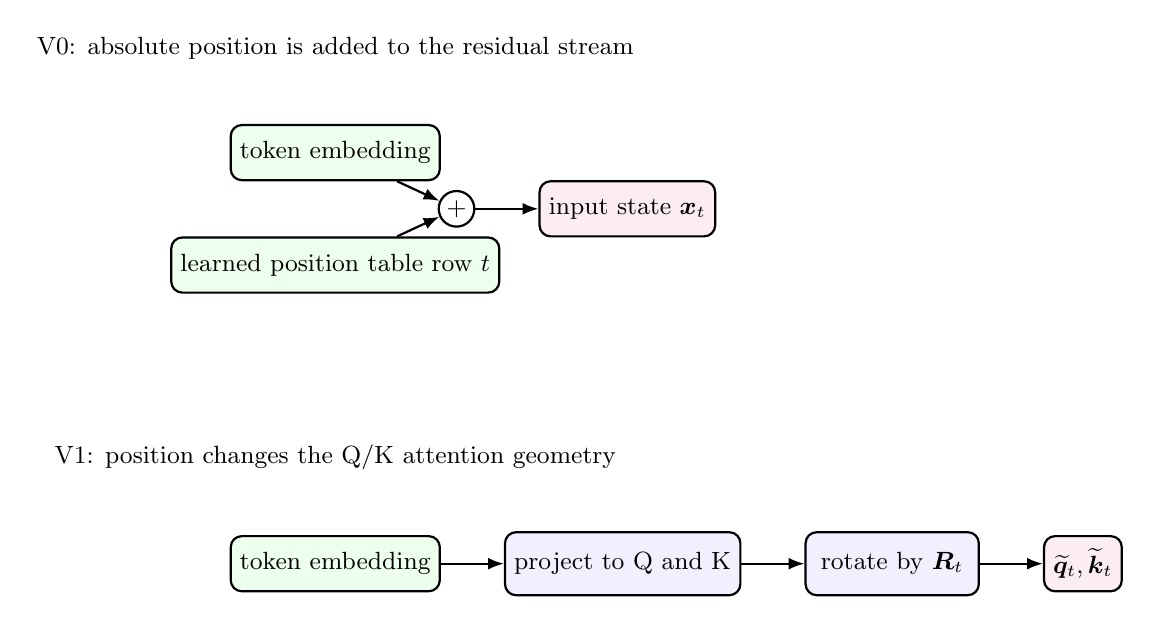
\begin{tikzpicture}[node distance=7mm and 8mm]
    \node[note] (v0title) {V0: absolute position is added to the residual stream};
    \node[data, below=of v0title] (tok) {token embedding};
    \node[data, below=of tok] (pos) {learned position table row $t$};
    \node[op, right=13mm of $(tok)!0.5!(pos)$] (add) {$+$};
    \node[tensor, right=of add] (x) {input state $\vx_t$};
    \draw[arrow] (tok) -- (add);
    \draw[arrow] (pos) -- (add);
    \draw[arrow] (add) -- (x);

    \node[note, below=18mm of pos] (v1title) {V1: position changes the Q/K attention geometry};
    \node[data, below=of v1title] (tok2) {token embedding};
    \node[block, right=of tok2] (proj) {project to Q and K};
    \node[block, right=of proj] (rot) {rotate by $\mR_t$};
    \node[tensor, right=of rot] (qk) {$\widetilde{\vq}_t,\widetilde{\vk}_t$};
    \draw[arrow] (tok2) -- (proj);
    \draw[arrow] (proj) -- (rot);
    \draw[arrow] (rot) -- (qk);
\end{tikzpicture}
\caption{Absolute embeddings versus RoPE. V0 injects position by addition to the residual stream; V1 injects position into the Q/K dot-product geometry.}
\label{fig:absolute-vs-rope}
\end{figure}

\begin{figure}[H]
\centering
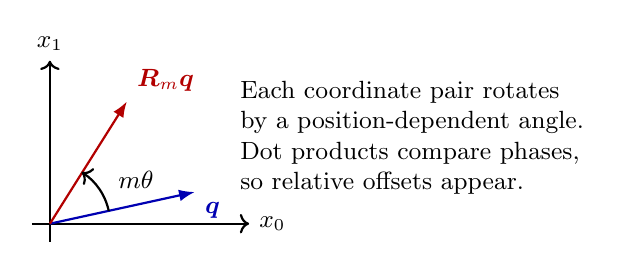
\begin{tikzpicture}[scale=1.15]
    \draw[->, thick] (-0.2,0) -- (2.2,0) node[right] {$x_0$};
    \draw[->, thick] (0,-0.2) -- (0,1.8) node[above] {$x_1$};
    \draw[arrow, blue!70!black] (0,0) -- (1.6,0.35) node[below right] {$\vq$};
    \draw[arrow, red!70!black] (0,0) -- (0.85,1.35) node[above right] {$\mR_m\vq$};
    \draw[->, thick] (0.65,0.14) arc[start angle=12,end angle=58,radius=0.67];
    \node[note] at (0.95,0.48) {$m\theta$};
    \node[note, align=left] at (4.0,0.95) {Each coordinate pair rotates\\by a position-dependent angle.\\Dot products compare phases,\\so relative offsets appear.};
\end{tikzpicture}
\caption{Two-dimensional RoPE rotation for one coordinate pair. The full head vector is partitioned into many such pairs with different frequencies.}
\label{fig:rope-rotation}
\end{figure}

\subsubsection{Frequency choice and long-context behavior}

The frequencies in \cref{eq:rope_freqs} form a geometric progression. Low-index coordinate pairs rotate quickly and can represent fine local offsets. High-index pairs rotate slowly and preserve phase information over longer distances. This multi-frequency design is analogous to using several sinusoidal scales.

RoPE gives a deterministic formula for positions beyond the training context, unlike a finite learned table. However, extrapolation is not guaranteed. High-frequency dimensions wrap many times at long contexts, and the model may see phase patterns outside the training distribution. Practical long-context variants often modify RoPE frequencies or scale positions.

\subsubsection{Why RoPE is applied to Q and K but not V}

Queries and keys determine routing: which token attends to which other token. Values contain content to be aggregated. Applying RoPE to Q and K makes attention scores position-aware. Applying it to V would rotate the content being averaged and is not necessary for relative-position routing.

\subsubsection{Trade-offs and implementation constraints}

RoPE introduces no learned position parameters and gives relative-offset structure in attention scores. The costs are implementation precision and extrapolation risk. The head dimension must be compatible with coordinate pairing, the same pairing convention must be used consistently, and cached keys must be rotated using exactly the same position convention as queries.

\begin{connectionbox}[Connection to no Q/K bias]
A fixed Q/K bias added before RoPE would be rotated by position, creating a position-dependent offset unrelated to token content. This is one reason RoPE-style models often remove Q/K biases. The detailed bias discussion appears once in \cref{sec:simplifications}.
\end{connectionbox}

\subsection{Component shift: explicit attention matrix to FlashAttention-style kernels}

\subsubsection{Baseline computation}

V0 attention materializes the full attention score matrix.
\begin{algorithm}[H]
\caption{Explicit causal self-attention}
\begin{algorithmic}[1]
\State $[\mQ;\mK;\mV]\gets \mX\mW_{\mathrm{qkv}}$ \Comment{shape $(B,T,3\dmodel)$}
\State reshape each tensor to $(B,\nhead,T,\dhead)$
\State $\mA\gets \mQ\mK^\top/\sqrt{\dhead}$ \Comment{shape $(B,\nhead,T,T)$}
\State set $A_{ij}\gets-\infty$ for $j>i$
\State $\mP\gets\softmax(\mA,\mathrm{dim}=-1)$
\State $\mO\gets\mP\mV$
\State concatenate heads and apply $\mW_O$
\end{algorithmic}
\end{algorithm}

The matrix has $B\nhead T^2$ entries. For $B=4$, $\nhead=8$, $T=2048$, and float32 storage, this is about $512$ MiB for one attention-probability tensor.

\subsubsection{Design pressure}

Longer contexts are useful only if the $T\times T$ attention matrix is feasible. The arithmetic cost of dense attention remains quadratic, but writing and reading the whole attention matrix from GPU high-bandwidth memory is a major bottleneck.

\subsubsection{Replacement mechanism}

FlashAttention computes the same attention function as \cref{eq:attention}, but avoids materializing the full $T\times T$ matrix in high-bandwidth memory. It uses tiling and an online softmax recurrence to keep only blocks of Q, K, V and running normalization statistics in faster on-chip memory \cite{dao2022flashattention}.

For one query row with score blocks $\vz^{(1)},\vz^{(2)},\ldots$, the online softmax maintains a running maximum $m$ and denominator $\ell$:
\begin{align}
    m_{\mathrm{new}}&=\max(m_{\mathrm{old}},\max_j z^{(b)}_j),\\
    \ell_{\mathrm{new}}&=
    e^{m_{\mathrm{old}}-m_{\mathrm{new}}}\ell_{\mathrm{old}}
    +\sum_j e^{z^{(b)}_j-m_{\mathrm{new}}}.
\end{align}
The partial weighted value sums are rescaled by the same factors, so the final result matches standard softmax attention up to floating-point associativity.

\begin{figure}[H]
\centering
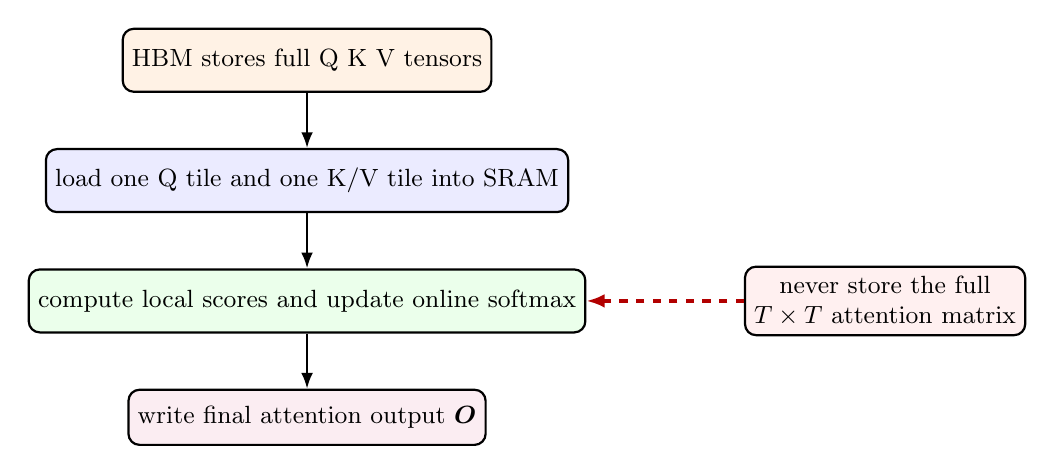
\begin{tikzpicture}[node distance=7mm and 8mm]
    \node[block, minimum width=42mm, fill=orange!10] (hbm) {HBM stores full Q K V tensors};
    \node[block, below=of hbm, minimum width=42mm, fill=blue!8] (load) {load one Q tile and one K/V tile into SRAM};
    \node[block, below=of load, minimum width=42mm, fill=green!8] (local) {compute local scores and update online softmax};
    \node[tensor, below=of local, minimum width=42mm] (out) {write final attention output $\mO$};
    \node[block, right=20mm of local, minimum width=34mm, fill=red!6] (avoid) {never store the full\\$T\times T$ attention matrix};

    \draw[arrow] (hbm) -- (load);
    \draw[arrow] (load) -- (local);
    \draw[arrow] (local) -- (out);
    \draw[grad] (avoid.west) -- (local.east);
\end{tikzpicture}
\caption{FlashAttention motivation. The mathematical attention output is the same, but the computation is tiled so the full attention matrix is not written to GPU high-bandwidth memory.}
\label{fig:flashattention}
\end{figure}

\subsubsection{Trade-off}

FlashAttention is a systems improvement, not a new statistical model. It reduces auxiliary memory and memory traffic, but it does not remove the $O(T^2\dhead)$ arithmetic cost of dense attention. It improves modeling results only indirectly when the saved memory or time is used for longer contexts, larger batches, or more training.

In PyTorch, V1 can call the fused scaled dot-product attention interface:
\begin{lstlisting}
out = F.scaled_dot_product_attention(
    q, k, v,
    attn_mask=None,
    dropout_p=dropout_p,
    is_causal=True,
)
\end{lstlisting}
Depending on hardware, dtype, tensor layout, and PyTorch version, this dispatches to a flash, memory-efficient, or math backend.


% =============================================================================
\section{Feed-Forward Networks: From ReLU/GELU to SwiGLU}
\label{sec:ffn}
% =============================================================================

\subsection{What the FFN does inside a Transformer block}

Attention answers a routing question: which earlier tokens should the current token read from? The feed-forward network answers a different question: after attention has gathered context, which new nonlinear features should be written back into the current token representation?

For a batch of hidden states $\mX\in\reals^{B\times T\times \dmodel}$, the FFN is applied independently at every position:
\begin{equation}
    \mathrm{FFN}(\mX)_{b,t,:}=g(\mX_{b,t,:}).
\end{equation}
This does \emph{not} mean the FFN ignores context. The vector $\mX_{b,t,:}$ has already been changed by attention, so it contains information gathered from previous tokens. The FFN transforms that contextual vector into new features.

\begin{intuitionbox}[One-token view]
For one token vector $\vx_t$, attention has already created a contextual summary such as ``this token is probably part of a noun phrase'', ``a closing bracket is expected'', or ``the previous word changes the meaning''. The FFN then turns this contextual information into new coordinates in the residual stream. In this sense, attention is communication, while the FFN is local computation after communication.
\end{intuitionbox}

\begin{figure}[H]
\centering
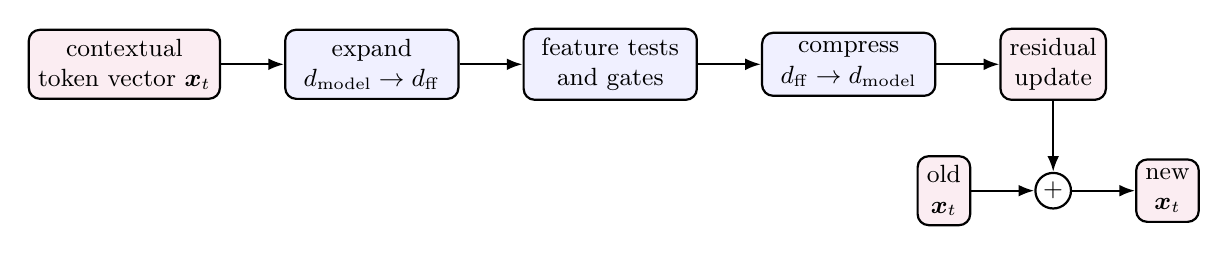
\begin{tikzpicture}[node distance=7mm and 8mm]
    \node[tensor] (x) {contextual\\token vector $\vx_t$};
    \node[block, right=of x] (expand) {expand\\$\dmodel\to\dff$};
    \node[block, right=of expand] (nonlin) {feature tests\\and gates};
    \node[block, right=of nonlin] (compress) {compress\\$\dff\to\dmodel$};
    \node[tensor, right=of compress] (update) {residual\\update};
    \node[op, below=9mm of update] (plus) {$+$};
    \node[tensor, left=of plus] (old) {old\\$\vx_t$};
    \node[tensor, right=of plus] (newx) {new\\$\vx_t$};

    \draw[arrow] (x) -- (expand);
    \draw[arrow] (expand) -- (nonlin);
    \draw[arrow] (nonlin) -- (compress);
    \draw[arrow] (compress) -- (update);
    \draw[arrow] (update) -- (plus);
    \draw[arrow] (old) -- (plus);
    \draw[arrow] (plus) -- (newx);
\end{tikzpicture}
\caption{The FFN writes a token-wise nonlinear update into the residual stream. The update should be expressive, but it must remain scale-compatible with residual addition. This is why FFN design connects to RMSNorm and residual-output initialization.}
\label{fig:ffn-residual-role}
\end{figure}

\subsection{The standard FFN as a collection of feature detectors}

The V0 FFN has the expand-activate-compress form
\begin{equation}\label{eq:standard_ffn}
    \mathrm{FFN}(\vx)=\mW_2\phi(\mW_1\vx),
\end{equation}
where $\mW_1\in\reals^{\dff\times\dmodel}$, $\mW_2\in\reals^{\dmodel\times\dff}$, and typically $\dff=4\dmodel$. If $\vw_i^\top$ is row $i$ of $\mW_1$ and $\vu_i$ is column $i$ of $\mW_2$, then
\begin{equation}
    a_i=\vw_i^\top\vx,
    \qquad
    h_i=\phi(a_i),
    \qquad
    \mathrm{FFN}(\vx)=\sum_{i=1}^{\dff}h_i\vu_i.
\end{equation}
This equation is the clearest way to understand an activation function. Hidden unit $i$ first asks whether the input vector $\vx$ matches a learned direction $\vw_i$. The answer is the pre-activation $a_i$. The activation function turns $a_i$ into a coefficient $h_i$. The output projection then writes $h_i$ times an output direction $\vu_i$ back into the residual stream.

\begin{motivationbox}[What an activation means inside a network]
When we say ``ReLU is zero for negative inputs'', the input is not usually a raw token or pixel. It is a learned score $a_i=\vw_i^\top\vx$. A positive score means ``the current residual-stream vector aligns with this learned feature direction.'' A negative score means ``it points away from this feature direction.'' ReLU turns this into a hard decision: aligned features are allowed to write; anti-aligned features write nothing.
\end{motivationbox}

\begin{example}[A simple hidden-unit example]
Suppose one FFN hidden unit has learned a direction $\vw_i$ that detects whether a contextual token vector looks like ``the start of a list item.'' If $a_i=\vw_i^\top\vx_t=2.0$, then ReLU outputs $2.0$, and the output direction $\vu_i$ is strongly written into the residual stream. If $a_i=-0.4$, ReLU outputs $0$, so this hidden unit contributes no update for that token. The unit is not choosing a token; it is choosing whether one learned feature should contribute to the next representation.
\end{example}

\subsection{Why ReLU helps}

\begin{definition}[Rectified Linear Unit]
\begin{equation}
    \ReLU(x)=\max(0,x)=x\ind[x>0].
\end{equation}
\end{definition}

ReLU helps neural networks for three basic reasons.

\paragraph{1. It makes the network nonlinear.}
Without activations, the composition of two linear maps is still one linear map:
\begin{equation}
    \mW_2(\mW_1\vx)=(\mW_2\mW_1)\vx.
\end{equation}
Stacking many such layers would not create a richer function class. ReLU breaks this collapse because different inputs activate different subsets of hidden units.

\paragraph{2. It creates input-dependent feature selection.}
For one input, hidden units $3,17,40$ might be active; for another input, units $2,9,51$ might be active. Thus the effective linear map changes with the input. A ReLU network is piecewise linear: it behaves like one linear model in one region of representation space and another linear model in another region.

\paragraph{3. It is cheap and sparse.}
ReLU requires only a comparison with zero. Also, inactive hidden units produce exact zeros. This can reduce unnecessary feature writing and was historically one reason ReLU became a strong baseline.

\begin{figure}[H]
\centering
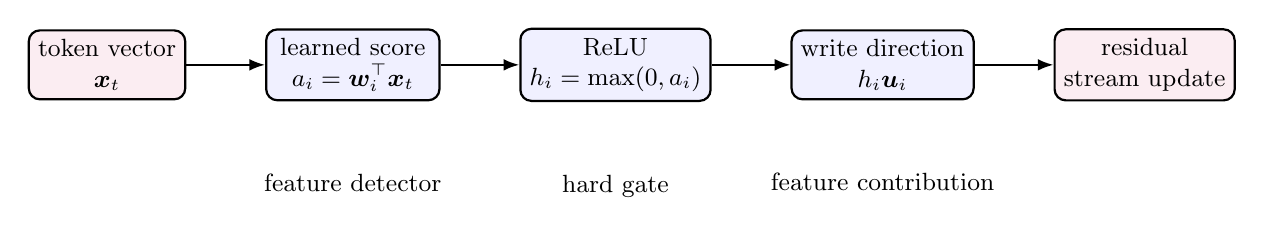
\begin{tikzpicture}[node distance=7mm and 10mm]
    \node[tensor] (x) {token vector\\$\vx_t$};
    \node[block, right=of x] (score) {learned score\\$a_i=\vw_i^\top\vx_t$};
    \node[block, right=of score] (relu) {ReLU\\$h_i=\max(0,a_i)$};
    \node[block, right=of relu] (write) {write direction\\$h_i\vu_i$};
    \node[tensor, right=of write] (resid) {residual\\stream update};
    \draw[arrow] (x) -- (score);
    \draw[arrow] (score) -- (relu);
    \draw[arrow] (relu) -- (write);
    \draw[arrow] (write) -- (resid);
    \node[note, below=8mm of score, align=center] {feature detector};
    \node[note, below=8mm of relu, align=center] {hard gate};
    \node[note, below=8mm of write, align=center] {feature contribution};
\end{tikzpicture}
\caption{A ReLU hidden unit inside an FFN. It is a learned feature detector followed by a hard gate and an output direction.}
\label{fig:relu-hidden-unit}
\end{figure}

\subsection{Why ReLU becomes limiting in Transformer FFNs}

The limitations of ReLU are easiest to see from the coefficient $h_i=\ReLU(a_i)$.

\paragraph{1. Negative evidence is erased.}
If $a_i=-2$, this is not weak evidence; it is strong evidence in the opposite direction. ReLU maps both $a_i=-2$ and $a_i=-0.01$ to the same value $0$. If the negative side is useful, the model must spend another hidden unit learning the opposite direction $-\vw_i$.

\paragraph{2. Inactive examples give zero local gradient.}
For $a_i<0$, $\ReLU'(a_i)=0$. During backpropagation, that particular example gives no direct gradient to the feature detector $\vw_i$. A ReLU unit is not guaranteed to be dead forever, because future batches or earlier layers may change $a_i$, but ReLU does create regions where the unit receives no local learning signal.

\paragraph{3. The hard threshold can waste capacity.}
A large Transformer FFN has many hidden units. If many units are inactive for many examples, the model has paid parameters for features that often do not contribute. Sparsity can be useful, but hard sparsity is not always the best use of parameters in a dense language model.

\paragraph{4. Feature selection and feature magnitude are tied.}
The same scalar $a_i$ decides both whether feature $i$ is allowed through and how large the contribution is. The FFN cannot separately learn ``what information is available'' and ``whether this context permits using it.'' This is the direct motivation for gated FFNs.

\begin{warningbox}[Careful wording]
It is too strong to say that ReLU neurons, once inactive, can never recover. The correct statement is local and example-specific: if $a_i<0$ for an example, the derivative through that ReLU is zero for that example. Across different batches and changing upstream representations, the unit may become active again.
\end{warningbox}

\subsection{GELU and SiLU: smoother single-path gates}

GELU and SiLU keep the same single-path FFN architecture but replace the hard ReLU gate by a smooth gate.

\begin{definition}[Gaussian Error Linear Unit]
\begin{equation}\label{eq:gelu}
    \GELU(x)=x\Phi(x),
\end{equation}
where $\Phi$ is the standard normal CDF.
\end{definition}

GELU can be read as ``multiply $x$ by a smooth probability-like measure of being positive.'' For large positive $x$, $\Phi(x)\approx 1$, so $\GELU(x)\approx x$. For large negative $x$, $\Phi(x)\approx 0$, so $\GELU(x)\approx 0$. Near zero, the transition is gradual rather than abrupt. Its derivative is
\begin{equation}
    \GELU'(x)=\Phi(x)+x\phi(x),
\end{equation}
where $\phi$ is the standard normal density. GELU was used in GPT-style models \cite{hendrycks2016gelu,radford2019gpt2}.

\begin{definition}[SiLU / Swish]
\begin{equation}\label{eq:silu}
    \SiLU(x)=x\sigma(x).
\end{equation}
\end{definition}

SiLU uses a logistic sigmoid gate instead of a Gaussian CDF gate. Its derivative is
\begin{equation}\label{eq:silu_derivative}
    \SiLU'(x)=\sigma(x)+x\sigma(x)(1-\sigma(x))
    =\sigma(x)\{1+x(1-\sigma(x))\}.
\end{equation}
SiLU allows small negative values to pass with reduced magnitude. It does not have an entire negative half-line with zero derivative, although the derivative can become very small and has an isolated zero at a negative value.

\begin{example}[Numerical intuition]
For $x=-1$, ReLU gives $0$, while SiLU gives approximately $-0.27$ and GELU gives approximately $-0.16$. Thus smooth activations do not say ``negative means impossible.'' They say ``negative evidence should usually be suppressed, but perhaps not deleted completely.'' For $x=2$, all three activations pass most of the value through, but GELU and SiLU still do so smoothly.
\end{example}

\begin{figure}[H]
\centering
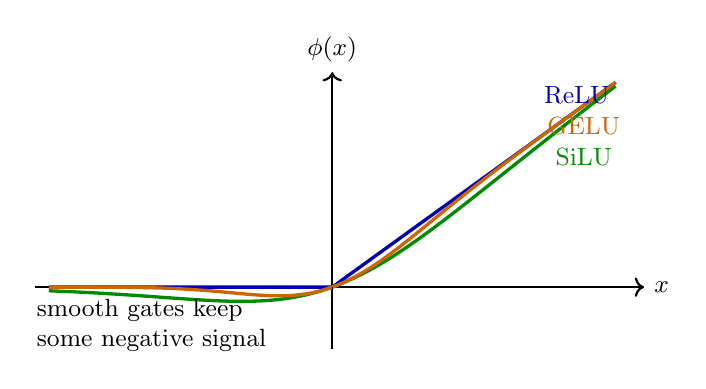
\begin{tikzpicture}[x=0.9cm,y=0.65cm]
    \draw[->, thick] (-4.2,0) -- (4.4,0) node[right] {$x$};
    \draw[->, thick] (0,-1.2) -- (0,4.2) node[above] {$\phi(x)$};
    \draw[very thick, blue!70!black] (-4,0) -- (0,0) -- (4,4);
    \draw[very thick, green!55!black, smooth, domain=-4:4, samples=120] plot (\x,{\x/(1+exp(-\x))});
    \draw[very thick, orange!80!black, smooth, domain=-4:4, samples=120] plot (\x,{0.5*\x*(1+tanh(0.7978845608*(\x+0.044715*\x*\x*\x)))});
    \draw[dashed] (0,0) -- (0,-0.9);
    \node[note, blue!70!black] at (3.45,3.75) {ReLU};
    \node[note, green!55!black] at (3.55,2.55) {SiLU};
    \node[note, orange!80!black] at (3.55,3.15) {GELU};
    \node[note, align=left] at (-2.55,-0.75) {smooth gates keep\\some negative signal};
\end{tikzpicture}
\caption{ReLU, GELU, and SiLU. GELU and SiLU are smoother single-path gates; they improve the activation curve but do not yet separate content from gating.}
\label{fig:relu-gelu-silu-shapes}
\end{figure}

\begin{connectionbox}[Why GELU and SiLU are only an intermediate step]
GELU and SiLU fix the hard-threshold problem, but they still use one projection. The same scalar both represents a candidate feature and decides how much of that feature should pass. SwiGLU changes the architecture by giving these two roles separate learned projections.
\end{connectionbox}

\subsection{SwiGLU: separating content from permission}

A gated FFN explicitly separates the two roles that ReLU combines:
\begin{equation}
    \text{content path: }\vu=\mW_{\mathrm{up}}\vx,
    \qquad
    \text{gate path: }\vg=\SiLU(\mW_{\mathrm{gate}}\vx).
\end{equation}
The SwiGLU FFN is
\begin{equation}\label{eq:swiglu}
    \mathrm{SwiGLU}(\vx)=
    \mW_{\mathrm{down}}\left[\SiLU(\mW_{\mathrm{gate}}\vx)\odot(\mW_{\mathrm{up}}\vx)\right].
\end{equation}
Here
\begin{equation}
    \mW_{\mathrm{gate}},\mW_{\mathrm{up}}\in\reals^{d_h\times\dmodel},
    \qquad
    \mW_{\mathrm{down}}\in\reals^{\dmodel\times d_h}.
\end{equation}
SwiGLU was proposed as one of several GLU variants for Transformer FFNs \cite{shazeer2020glu} and is used in LLaMA-style architectures \cite{touvron2023llama}.

\begin{motivationbox}[Why the project swaps ReLU/GELU to SwiGLU]
The project swaps to SwiGLU because the FFN should do more than ask whether one learned scalar is positive. It should learn conditional feature computation: ``this content is available, and this context decides how much of it should be written.'' The up path supplies candidate content; the gate path supplies context-dependent permission; their product performs feature-wise selection.
\end{motivationbox}

\begin{figure}[H]
\centering
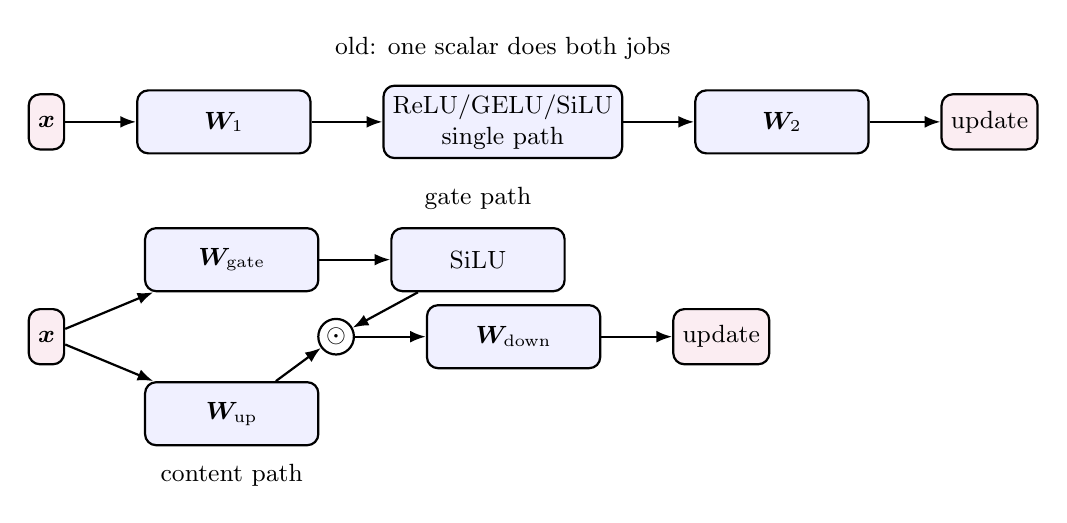
\begin{tikzpicture}[node distance=8mm and 9mm]
    \node[tensor] (x1) {$\vx$};
    \node[block, right=of x1] (w1) {$\mW_1$};
    \node[block, right=of w1] (relu) {ReLU/GELU/SiLU\\single path};
    \node[block, right=of relu] (w2) {$\mW_2$};
    \node[tensor, right=of w2] (out1) {update};

    \node[tensor, below=20mm of x1] (x2) {$\vx$};
    \node[block, above right=2mm and 10mm of x2] (wg) {$\mW_{\mathrm{gate}}$};
    \node[block, right=of wg] (sg) {SiLU};
    \node[block, below right=2mm and 10mm of x2] (wu) {$\mW_{\mathrm{up}}$};
    \node[op, right=32mm of x2] (mul) {$\odot$};
    \node[block, right=of mul] (wd) {$\mW_{\mathrm{down}}$};
    \node[tensor, right=of wd] (out2) {update};

    \draw[arrow] (x1) -- (w1);
    \draw[arrow] (w1) -- (relu);
    \draw[arrow] (relu) -- (w2);
    \draw[arrow] (w2) -- (out1);

    \draw[arrow] (x2) -- (wg);
    \draw[arrow] (wg) -- (sg);
    \draw[arrow] (sg) -- (mul);
    \draw[arrow] (x2) -- (wu);
    \draw[arrow] (wu) -- (mul);
    \draw[arrow] (mul) -- (wd);
    \draw[arrow] (wd) -- (out2);

    \node[note, above=2mm of relu] {old: one scalar does both jobs};
    \node[note, below=1mm of wu] {content path};
    \node[note, above=1mm of sg] {gate path};
\end{tikzpicture}
\caption{The core ReLU-to-SwiGLU shift. ReLU/GELU/SiLU use one hidden path; SwiGLU separates candidate content from the gate that decides how much content to write.}
\label{fig:relu-to-swiglu}
\end{figure}

\begin{example}[A simple gate-content example]
Suppose the content path proposes $u_i=5$, meaning ``write a strong feature in direction $\vu_i$.'' If the gate is $g_i=0.05$, the product is $0.25$, so the feature is almost suppressed. If the gate is $g_i=1.8$, the product is $9$, so the feature is amplified. The important point is that the model can learn content and permission separately: the content may be useful, but only under certain contexts.
\end{example}

\subsection{Advantages of SwiGLU over ReLU/GELU}

\paragraph{1. Smooth gating.}
The gate uses SiLU, so the transition from suppressed to active is smooth rather than a hard half-line cutoff.

\paragraph{2. Separate content and selection.}
The up projection can specialize in candidate features, while the gate projection can specialize in deciding which candidate features matter for the current context.

\paragraph{3. Multiplicative interactions.}
The product $\vg\odot\vu$ creates conditional interactions between two learned projections. A plain ReLU FFN can approximate such effects, but SwiGLU represents them more directly.

\paragraph{4. Parameter-efficient quality.}
When the hidden dimension is adjusted so that parameter count is comparable, gated variants such as SwiGLU have empirically improved Transformer FFNs over ReLU/GELU baselines \cite{shazeer2020glu}. The fair comparison is parameter-matched, not width-matched.

\paragraph{5. Good fit with pre-normalized residual blocks.}
RMSNorm controls the scale of $\vx$ before the gate and content projections. Residual-output initialization controls the scale of $\mW_{\mathrm{down}}$ when writing the gated update back into the residual stream. Thus SwiGLU is not isolated; it relies on the surrounding architecture to keep multiplicative updates stable.

\subsection{Costs introduced by SwiGLU}

\begin{tradeoffbox}[SwiGLU is not free]
SwiGLU improves expressivity, but it introduces costs.
\begin{enumerate}[nosep]
    \item \textbf{Extra projection:} ReLU/GELU FFNs use two matrices; SwiGLU uses three.
    \item \textbf{Activation memory:} the gate and content activations may both be stored for backpropagation.
    \item \textbf{Less exact sparsity:} ReLU gives exact zeros; SiLU gates are usually nonzero.
    \item \textbf{Scale sensitivity:} multiplying two learned projections can increase activation variance if not controlled.
    \item \textbf{More design choices:} the hidden dimension $d_h$ must be chosen and often rounded to a hardware-friendly multiple.
\end{enumerate}
\end{tradeoffbox}

\subsection{Parameter matching: why the hidden width changes}

The standard FFN with $\dff=4\dmodel$ has
\begin{equation}
    2\dmodel\dff=8\dmodel^2
\end{equation}
parameters. SwiGLU has three matrices:
\begin{equation}
    3\dmodel d_h.
\end{equation}
Matching total parameter count gives
\begin{equation}
    3\dmodel d_h=8\dmodel^2
    \qquad\Rightarrow\qquad
    d_h=\frac{8}{3}\dmodel.
\end{equation}
In code, $d_h$ is often rounded to a multiple such as $64$ or $256$ for efficient tensor-core use.

\begin{figure}[H]
\centering
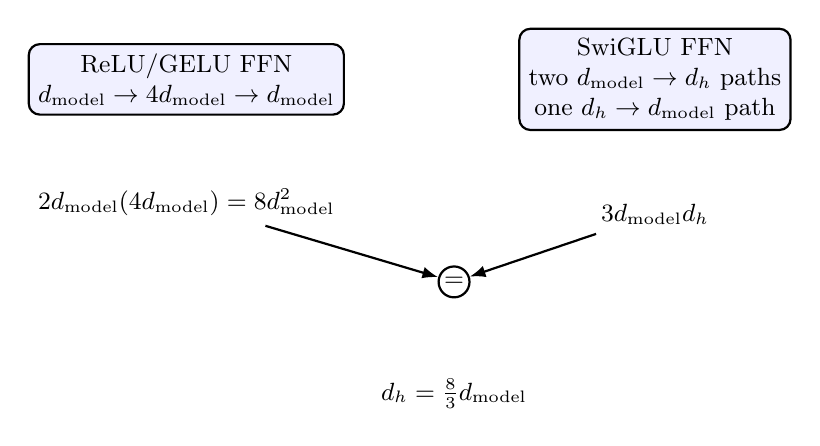
\begin{tikzpicture}[node distance=9mm and 8mm]
    \node[block] (relu) {ReLU/GELU FFN\\$\dmodel\to4\dmodel\to\dmodel$};
    \node[block, right=22mm of relu] (swiglu) {SwiGLU FFN\\two $\dmodel\to d_h$ paths\\one $d_h\to\dmodel$ path};
    \node[note, below=8mm of relu] (p1) {$2\dmodel(4\dmodel)=8\dmodel^2$};
    \node[note, below=8mm of swiglu] (p2) {$3\dmodel d_h$};
    \node[op, below=19mm of relu, xshift=34mm] (eq) {$=$};
    \node[note, below=9mm of eq] {$d_h=\frac{8}{3}\dmodel$};
    \draw[arrow] (p1) -- (eq);
    \draw[arrow] (p2) -- (eq);
\end{tikzpicture}
\caption{Parameter matching for ReLU/GELU FFN versus SwiGLU FFN. SwiGLU spends parameters on a separate gate path, so the hidden width is reduced from $4\dmodel$ to about $(8/3)\dmodel$.}
\label{fig:swiglu-param-matching}
\end{figure}

\subsection{Implementation}

\begin{lstlisting}
gate = F.silu(self.w_gate(x))   # gate path: decides what to pass
up = self.w_up(x)               # content path: candidate features
hidden = gate * up              # multiplicative feature selection
out = self.w_down(hidden)       # write update back to residual stream
\end{lstlisting}

\begin{connectionbox}[One-sentence summary]
ReLU is a hard one-path feature detector; GELU and SiLU are smoother one-path gates; SwiGLU is a two-path gated FFN that separates candidate content from context-dependent permission, at the cost of another projection and more activation memory.
\end{connectionbox}


% =============================================================================
\section{Autoregressive Generation and Decoding}
\label{sec:generation}
% =============================================================================

Training and generation use the same conditional distribution,
\begin{equation}
    p_{\vtheta}(s_{t+1}\given s_{1:t}),
\end{equation}
but they use it differently. Training evaluates many positions in parallel and compares them with known next tokens. Generation has no future tokens available; it repeatedly samples or selects one token, appends it to the context, and runs the model again.

\subsection{Why naive generation repeats work}

At generation step $t$, a naive implementation feeds the whole prefix $s_{1:t}$ through every layer again. This recomputes hidden states, keys, and values for all earlier positions, even though those earlier tokens have not changed. The waste is easiest to see from causal attention: the key and value at position $j$ depend only on $s_{\leq j}$, because the causal mask prevents dependence on future tokens. Therefore, once $\vk_j$ and $\vv_j$ are computed, future tokens cannot invalidate them.

\begin{intuitionbox}[Caching in ordinary language]
If you have already summarized chapter 1 of a book, you do not need to re-summarize chapter 1 from scratch every time you read a new sentence in chapter 2. You keep the old summary and add the new information. The KV-cache is the Transformer's version of keeping old summaries: it stores old keys and values so the new query can read from them.
\end{intuitionbox}

\subsection{KV-cache definition and mechanism}

\begin{definition}[KV-cache]
For each layer $\ell$, the KV-cache stores the keys and values already computed for previous positions:
\begin{equation}
    \mathrm{cache}^{(\ell)}_t=\left(\mK^{(\ell)}_{1:t},\mV^{(\ell)}_{1:t}\right).
\end{equation}
At step $t+1$, the model computes only $\vq_{t+1},\vk_{t+1},\vv_{t+1}$ for the new token, appends $\vk_{t+1},\vv_{t+1}$ to the cache, and attends the new query to all cached keys and values.
\end{definition}

\begin{figure}[H]
\centering
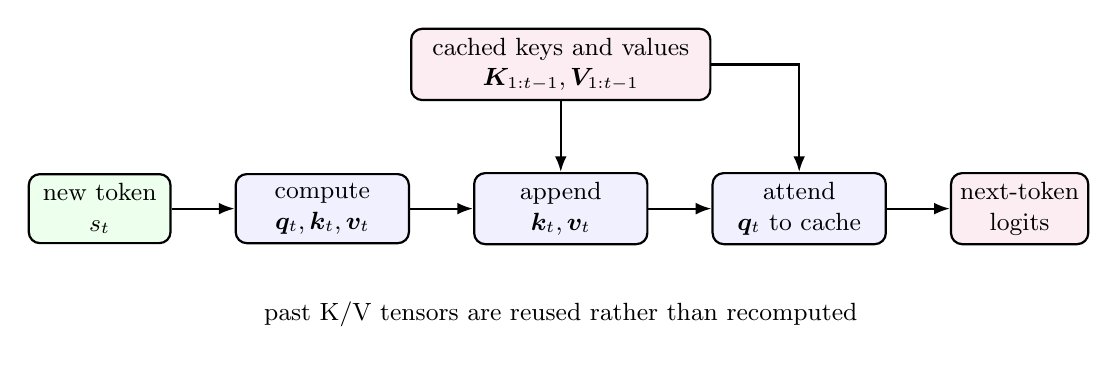
\begin{tikzpicture}[node distance=7mm and 8mm]
    \node[data] (new) {new token\\$s_t$};
    \node[block, right=of new] (proj) {compute\\$\vq_t,\vk_t,\vv_t$};
    \node[block, right=of proj] (append) {append\\$\vk_t,\vv_t$};
    \node[tensor, above=9mm of append, minimum width=38mm] (cache) {cached keys and values\\$\mK_{1:t-1},\mV_{1:t-1}$};
    \node[block, right=of append] (attn) {attend\\$\vq_t$ to cache};
    \node[tensor, right=of attn] (out) {next-token\\logits};

    \draw[arrow] (new) -- (proj);
    \draw[arrow] (proj) -- (append);
    \draw[arrow] (cache) -- (append);
    \draw[arrow] (append) -- (attn);
    \draw[arrow] (cache) -| (attn);
    \draw[arrow] (attn) -- (out);
    \node[note, below=6mm of append] {past K/V tensors are reused rather than recomputed};
\end{tikzpicture}
\caption{KV-cache during autoregressive generation. The new query reads from stored keys and values from previous positions.}
\label{fig:kv-cache}
\end{figure}

\subsection{Compute, memory, and limitations of the KV-cache}

The KV-cache does not remove the need to attend over previous tokens. The new query still compares itself with $t$ cached keys. The gain is that the model does not recompute old hidden states and old K/V projections.

The cache memory across all layers is
\begin{equation}\label{eq:kvcache_memory}
    2\cdot\nlayer\cdot B\cdot\nhead\cdot T\cdot\dhead\cdot s,
\end{equation}
where the factor $2$ is for K and V, and $s$ is bytes per element. Since $\nhead\dhead=\dmodel$ for standard MHA, this is also
\begin{equation}
    2\cdot\nlayer\cdot B\cdot T\cdot\dmodel\cdot s.
\end{equation}

\begin{example}[Cache size]
For $\nlayer=8$, $B=1$, $\nhead=8$, $T=1024$, $\dhead=64$, and bf16 ($s=2$ bytes), the cache uses
\begin{equation}
    2\cdot8\cdot1\cdot8\cdot1024\cdot64\cdot2=16\text{ MiB}.
\end{equation}
This is small for one sequence, but it grows linearly with batch size, generated length, and number of simultaneous users.
\end{example}

\begin{tradeoffbox}[KV-cache trade-off]
The KV-cache changes inference computation but not the learned distribution. It buys speed by spending memory. Long-context serving is often limited by cache memory rather than by the parameter memory of the model itself.
\end{tradeoffbox}

\subsection{KV-cache with RoPE}

With RoPE, keys are stored after rotation:
\begin{equation}
    \vk_t=\mW_K\vx_t,
    \qquad
    \widetilde{\vk}_t=\mR_t\vk_t.
\end{equation}
The cache stores $\widetilde{\vk}_t$. Future queries are rotated by their own positions and compared against already rotated keys. No old key needs to be re-rotated.

\begin{connectionbox}[Why RoPE and caching fit together]
RoPE applies a deterministic position-dependent rotation to each key at creation time. Since causal attention makes old keys independent of future tokens, the rotated key remains valid forever. This is why the correct generation order is: project K, rotate K by its position, then store it in the cache.
\end{connectionbox}

\subsection{A note on MQA and GQA}

This project uses standard multi-head attention unless stated otherwise. Production LLMs often use multi-query attention (MQA) or grouped-query attention (GQA), where several query heads share fewer key/value heads. These variants reduce cache memory by replacing $\nhead$ K/V heads with $n_{\mathrm{kv}}<\nhead$ K/V heads:
\begin{equation}
    \mathrm{cache\ memory}\propto n_{\mathrm{kv}}\dhead
    \quad\text{instead of}\quad
    \nhead\dhead.
\end{equation}
MQA and GQA should be documented as future attention-serving variants, not as part of the current V1 shift.

\subsection{From logits to a generated token}

After the model produces logits $\vz\in\reals^{\vocab}$, decoding converts those scores into the next token. This is not part of training; it is a decision rule applied to the trained probability distribution. Different decoding rules can make the same model look deterministic, creative, repetitive, or noisy.

\begin{example}[Toy next-token distribution]
Suppose the model gives the following probabilities after the prompt ``The cat sat on the'':
\begin{center}
\begin{tabular}{lcccccc}
\toprule
Token & mat & floor & sofa & roof & banana & quantum\\
\midrule
Probability & 0.42 & 0.24 & 0.16 & 0.08 & 0.06 & 0.04\\
\bottomrule
\end{tabular}
\end{center}
Greedy decoding always picks ``mat''. Sampling may pick ``floor'' or ``sofa'' sometimes. Top-$k$ and top-$p$ decide which low-probability tokens are allowed into the sampling set.
\end{example}

\begin{figure}[H]
\centering
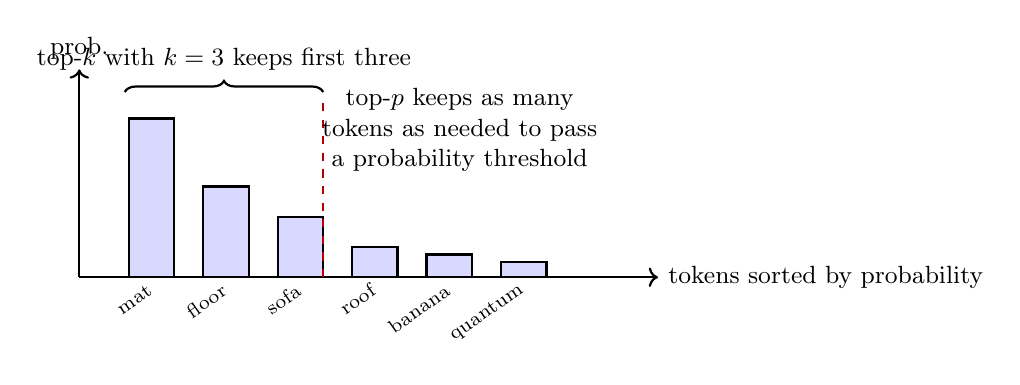
\begin{tikzpicture}[x=1.05cm,y=4.8cm]
    \draw[->, thick] (0,0) -- (7,0) node[right] {tokens sorted by probability};
    \draw[->, thick] (0,0) -- (0,0.55) node[above] {prob.};
    \foreach \x/\h/\lab in {0.6/0.42/mat,1.5/0.24/floor,2.4/0.16/sofa,3.3/0.08/roof,4.2/0.06/banana,5.1/0.04/quantum}{
        \draw[fill=blue!15, thick] (\x,0) rectangle +(0.55,\h);
        \node[rotate=35, anchor=east, font=\scriptsize] at (\x+0.35,-0.015) {\lab};
    }
    \draw[decorate,decoration={brace,amplitude=4pt},thick] (0.55,0.49) -- node[above=4pt, note] {top-$k$ with $k=3$ keeps first three} (2.95,0.49);
    \draw[dashed, red!70!black, thick] (2.95,0) -- (2.95,0.47);
    \node[note, align=center] at (4.6,0.39) {top-$p$ keeps as many\\tokens as needed to pass\\a probability threshold};
\end{tikzpicture}
\caption{Decoding filters operate on the probability distribution after the model has been trained. They change generation behavior but not the model parameters.}
\label{fig:decoding-filters}
\end{figure}

\subsection{Temperature scaling}

Temperature rescales logits before softmax:
\begin{equation}
    p_i(\tau)=\frac{\exp(z_i/\tau)}{\sum_j\exp(z_j/\tau)}.
\end{equation}
For $\tau<1$, the distribution becomes sharper. For $\tau>1$, the distribution becomes flatter. As $\tau\to0$, sampling approaches greedy decoding.

\begin{intuitionbox}[Temperature as confidence control]
Temperature does not change the ranking of tokens; it changes how strongly the model prefers high-ranked tokens. Low temperature says ``trust the model's favorite choices strongly.'' High temperature says ``allow more alternatives.'' Very high temperature can make output incoherent because low-probability tokens become too likely.
\end{intuitionbox}

\subsection{Greedy decoding}

Greedy decoding chooses the most likely next token:
\begin{equation}
    s_{t+1}=\argmax_w p_{\vtheta}(w\given s_{\leq t}).
\end{equation}
It is deterministic and fast. Its limitation is that local probability maximization can lead to repetitive or bland text. The most likely next token at each step is not necessarily part of the best full sequence.

\subsection{Top-$k$ sampling}

Top-$k$ keeps only the $k$ highest-probability tokens:
\begin{equation}
    p_{\mathrm{top}\text{-}k}(w)=\begin{cases}
        p(w)/\sum_{u\in S_k}p(u), & w\in S_k,\\
        0, & w\notin S_k,
    \end{cases}
\end{equation}
where $S_k$ is the set of $k$ highest-probability tokens.

\begin{example}[Top-$k$ on the toy distribution]
With $k=3$, the allowed tokens are ``mat'', ``floor'', and ``sofa''. The other tokens receive probability zero. The remaining probabilities are renormalized: the new probability of ``mat'' is $0.42/(0.42+0.24+0.16)\approx0.51$.
\end{example}

The limitation is that $k$ is fixed. If the model is very confident, $k=50$ may include many implausible tokens. If the model is uncertain, $k=50$ may exclude reasonable options.

\subsection{Nucleus sampling or top-$p$ sampling}

Nucleus sampling sorts tokens by descending probability and chooses the smallest prefix $S_p$ whose cumulative probability is at least $p$ \cite{holtzman2019nucleus}:
\begin{equation}
    S_p=\min\left\{S:\sum_{w\in S}p(w)\geq p\right\},
\end{equation}
where the minimum is over prefixes of the sorted token list. Then the distribution is renormalized over $S_p$.

\begin{example}[Top-$p$ on the toy distribution]
If $p=0.8$, we include ``mat'' ($0.42$), ``floor'' ($0.66$ cumulative), and ``sofa'' ($0.82$ cumulative). We stop after ``sofa'' because the cumulative probability has passed $0.8$. If the distribution were flatter, top-$p$ would automatically include more tokens.
\end{example}

\subsection{Decoding is not training}

\begin{motivationbox}[Separate the learned distribution from the decision rule]
Training estimates conditional probabilities by minimizing cross-entropy. Decoding chooses how to use those probabilities. A model can have a lower validation loss but still produce poor samples under a bad decoding rule. Conversely, careful temperature and top-$p$ settings can make a fixed model sound much better without changing its learned parameters.
\end{motivationbox}

Common sampling hyperparameters should therefore be reported with generation examples: temperature, top-$k$, top-$p$, maximum length, repetition penalties if used, and the prompt format.


% =============================================================================
\section{Architectural Simplifications}
\label{sec:simplifications}
% =============================================================================

This section contains smaller architecture choices from the original notes. They should not be re-explained elsewhere: if a future variant changes one of them, add the explanation here.

\subsection{Weight tying}

\begin{definition}[Weight tying]
The input embedding matrix and output classifier matrix share parameters:
\begin{equation}
    \mW_{\mathrm{head}}=\mW_{\mathrm{tok}}.
\end{equation}
\end{definition}
The logit for token $w$ becomes
\begin{equation}
    z_w=\vh^\top\mW_{\mathrm{tok}}[w].
\end{equation}
Thus the model uses the same vector space for reading tokens and predicting tokens. If the final hidden vector $\vh$ points in a similar direction to the embedding of token $w$, then token $w$ receives a large logit.

\begin{example}[Why tying saves parameters]
If $\vocab=50{,}000$ and $\dmodel=512$, the embedding matrix has about $25.6$ million parameters. Without weight tying, the output head would add another $25.6$ million parameters. Tying shares these parameters and also encourages a consistent geometry between input tokens and output predictions.
\end{example}

Weight tying can significantly reduce parameters when $\vocab\dmodel$ is large \cite{press2017weighttying}. Its limitation is that it constrains the input and output token spaces to use the same embedding geometry. In language modeling this is usually beneficial, but it is still a modeling assumption.

\subsection{Mostly bias-free layers}

A standard linear layer uses $\mW\vx+\bm b$. Modern decoder-only LLMs often omit biases in most projections:
\begin{equation}
    \vy=\mW\vx.
\end{equation}
The motivation is practical, not mystical. Bias vectors are small compared with large matrices, and pre-normalization already controls the distribution entering each projection. For Q/K projections with RoPE, bias terms are especially awkward: a fixed vector added before rotation becomes a position-dependent rotated offset.

\begin{connectionbox}[Connection to RMSNorm and RoPE]
RMSNorm uses scale without an additive shift. Bias-free projections extend the same minimalist style. RoPE wants position to enter through rotations of Q and K; removing Q/K biases keeps that geometry cleaner.
\end{connectionbox}

The trade-off is reduced affine flexibility. Bias-free layers are a modern LLM convention, not a theorem that biases are never useful. Small-data fine-tuning or non-language tasks may benefit from biases.

\subsection{No-dropout pretraining}

\begin{definition}[Dropout]
During training, dropout sets activations to zero with probability $p$ and rescales surviving activations:
\begin{equation}
    \mathrm{Dropout}(x_i)=\begin{cases}
        0, & \text{with probability }p,\\
        x_i/(1-p), & \text{with probability }1-p.
    \end{cases}
\end{equation}
\end{definition}

Dropout is a regularizer. It is useful when a model can overfit a limited dataset by relying on fragile co-adapted features. Large-scale pretraining often uses zero dropout because the limiting factor is usually not classical small-data overfitting; it is efficient use of data, compute, and optimization.

\begin{tradeoffbox}[When no dropout can fail]
No-dropout pretraining is not a universal rule. If the training loss keeps decreasing while validation loss increases, the model is overfitting and dropout or another regularizer may help. For fair V0/V1 comparisons, dropout should be fixed across variants unless dropout is the object of the experiment.
\end{tradeoffbox}

% =============================================================================
\section{Training, Numerical Precision, and Evaluation}
\label{sec:training-eval}
% =============================================================================

\subsection{AdamW and weight-decay groups}

Adam keeps moving averages of gradients and squared gradients:
\begin{align}
    \bm m_t&=\beta_1\bm m_{t-1}+(1-\beta_1)\bm g_t,\\
    \bm v_t&=\beta_2\bm v_{t-1}+(1-\beta_2)\bm g_t^2.
\end{align}
Bias-corrected estimates are
\begin{equation}
    \widehat{\bm m}_t=\frac{\bm m_t}{1-\beta_1^t},
    \qquad
    \widehat{\bm v}_t=\frac{\bm v_t}{1-\beta_2^t}.
\end{equation}
AdamW decouples weight decay from the adaptive gradient scaling \cite{loshchilov2019adamw}:
\begin{equation}\label{eq:adamw}
    \vtheta_t=\vtheta_{t-1}
    -\eta_t\frac{\widehat{\bm m}_t}{\sqrt{\widehat{\bm v}_t}+\epsilon}
    -\eta_t\lambda\vtheta_{t-1}.
\end{equation}
A common rule is to apply weight decay to two-dimensional weight matrices, but not to normalization scales, embeddings, or bias vectors.

\subsection{Learning-rate warmup and cosine decay}

A standard schedule is
\begin{equation}\label{eq:cosine_schedule}
    \eta(t)=\begin{cases}
        \eta_{\max}\,t/t_{\mathrm{warmup}}, & t<t_{\mathrm{warmup}},\\[0.5em]
        \eta_{\min}+\dfrac{\eta_{\max}-\eta_{\min}}{2}
        \left(1+\cos\left(\pi\dfrac{t-t_{\mathrm{warmup}}}{t_{\mathrm{total}}-t_{\mathrm{warmup}}}\right)\right), & t\geq t_{\mathrm{warmup}}.
    \end{cases}
\end{equation}
Warmup avoids unstable early updates before Adam's moment estimates are calibrated. Decay reduces optimization noise later.

\begin{figure}[H]
\centering
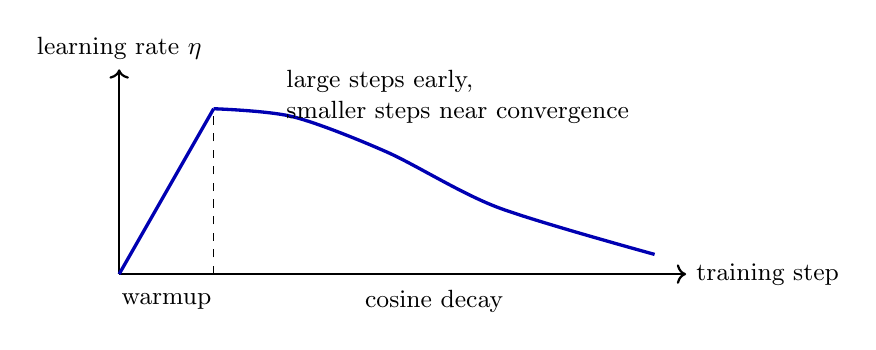
\begin{tikzpicture}[x=1cm,y=1cm]
    \draw[->, thick] (0,0) -- (7.2,0) node[right] {training step};
    \draw[->, thick] (0,0) -- (0,2.6) node[above] {learning rate $\eta$};
    \draw[very thick, blue!70!black] (0,0) -- (1.2,2.1);
    \draw[very thick, blue!70!black] plot[smooth] coordinates {(1.2,2.1) (2.2,2.0) (3.4,1.55) (4.8,0.85) (6.8,0.25)};
    \draw[dashed] (1.2,0) -- (1.2,2.1);
    \node[note] at (0.6,-0.35) {warmup};
    \node[note] at (4.0,-0.35) {cosine decay};
    \node[note, align=left] at (4.3,2.25) {large steps early,\\smaller steps near convergence};
\end{tikzpicture}
\caption{Learning-rate warmup and decay. The schedule is part of a fair architecture comparison because a bad schedule can hide the value of an architecture.}
\label{fig:lr-schedule}
\end{figure}

\subsection{Gradient clipping and accumulation}

Global norm clipping rescales the full gradient vector if it exceeds threshold $c$:
\begin{equation}\label{eq:grad_clip}
    \bm g\leftarrow \bm g\cdot\min\left(1,\frac{c}{\Vert\bm g\Vert_2}\right).
\end{equation}
This preserves direction when clipping occurs and protects against rare destructive updates.

If the desired effective batch size does not fit in memory, use $A$ micro-batches:
\begin{equation}
    \bm g_{\mathrm{eff}}=\frac{1}{A}\sum_{a=1}^{A}\bm g^{(a)}.
\end{equation}
The optimizer steps once after accumulating $A$ gradients. Usually each micro-batch loss is divided by $A$ before backpropagation.

\subsection{Mixed precision and bfloat16}

\begin{center}
\begin{tabular}{lcccc}
\toprule
Format & Sign bits & Exponent bits & Mantissa bits & Total bits\\
\midrule
float32 & 1 & 8 & 23 & 32\\
float16 & 1 & 5 & 10 & 16\\
bfloat16 & 1 & 8 & 7 & 16\\
\bottomrule
\end{tabular}
\end{center}

bfloat16 has the same exponent width as float32, so it has a much larger dynamic range than float16. Its mantissa is shorter, so individual numbers are less precise, but neural-network gradients are already noisy because they are estimated from mini-batches. In practice, the larger exponent range is often more important than extra mantissa bits.

\begin{intuitionbox}[Why bf16 works]
Mini-batch training already uses an approximate gradient. If the stochastic error from sampling a batch is larger than the rounding error from bf16 arithmetic, then bf16 matrix multiplications can be a good trade-off. However, reductions such as softmax denominators, normalization statistics, and losses are more sensitive to accumulation error, so they are often kept in float32.
\end{intuitionbox}

A typical mixed-precision strategy is:
\begin{itemize}[nosep]
    \item matrix multiplications in bf16 for speed and memory bandwidth;
    \item softmax, normalization reductions, and loss accumulation in float32;
    \item Adam moments and sometimes master weights in float32.
\end{itemize}

\subsection{Scaling-law perspective}

For a fixed compute budget, increasing model size without increasing training tokens can be inefficient. Compute-optimal scaling analyses suggest that model size and data size should be balanced rather than scaling only parameters \cite{hoffmann2022chinchilla}. For this project, if V1 improves validation loss over V0, the comparison should control for training tokens, optimizer settings, context length, and parameter count.

\subsection{Fair V0 versus V1 comparison}

To attribute performance differences to architecture rather than confounders, keep the following fixed:
\begin{itemize}[nosep]
    \item tokenizer and vocabulary;
    \item training and validation data;
    \item number of training tokens;
    \item context length;
    \item optimizer and learning-rate schedule;
    \item token batch size;
    \item parameter count, as closely as possible.
\end{itemize}

\begin{figure}[H]
\centering
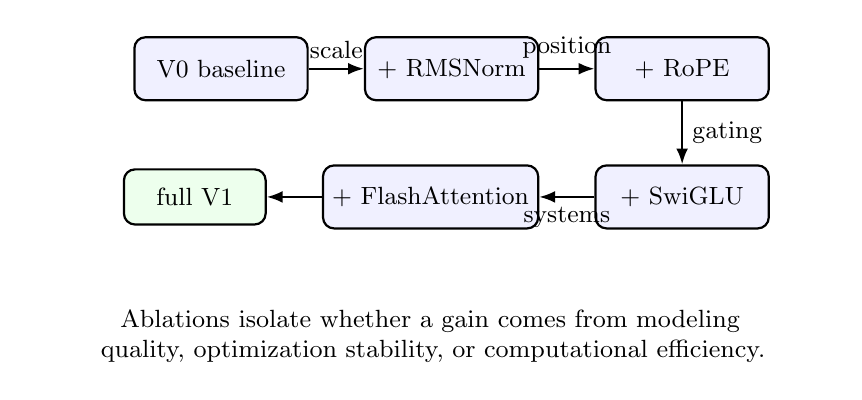
\begin{tikzpicture}[node distance=8mm and 7mm]
    \node[block] (v0) {V0 baseline};
    \node[block, right=of v0] (rms) {+ RMSNorm};
    \node[block, right=of rms] (rope) {+ RoPE};
    \node[block, below=of rope] (swiglu) {+ SwiGLU};
    \node[block, left=of swiglu] (flash) {+ FlashAttention};
    \node[data, left=of flash] (v1) {full V1};

    \draw[arrow] (v0) -- node[above, note] {scale} (rms);
    \draw[arrow] (rms) -- node[above, note] {position} (rope);
    \draw[arrow] (rope) -- node[right, note] {gating} (swiglu);
    \draw[arrow] (swiglu) -- node[below, note] {systems} (flash);
    \draw[arrow] (flash) -- (v1);
    \node[note, below=9mm of flash, align=center, text width=10cm] {Ablations isolate whether a gain comes from modeling quality, optimization stability, or computational efficiency.};
\end{tikzpicture}
\caption{Ablation path for a meaningful V0-to-V1 comparison. FlashAttention should mainly change speed and memory; RoPE, RMSNorm, and SwiGLU may affect loss.}
\label{fig:ablation-path}
\end{figure}

\subsection{Validation uncertainty, sanity checks, and calibration}

Token losses are correlated within documents, so a simple token-level standard error is too optimistic. A rougher batch- or document-level estimate is
\begin{equation}
    \mathrm{SE}(\widehat R)\approx \frac{s_{\mathrm{batch}}}{\sqrt{n_{\mathrm{batch}}}},
\end{equation}
where $s_{\mathrm{batch}}$ is the sample standard deviation of batch-level losses.

Before trusting a training run, verify:
\begin{enumerate}[nosep]
    \item loss at initialization is near $\log\vocab$ when logits are close to uniform;
    \item the model can overfit a tiny batch;
    \item predictions at position $t$ do not change when future tokens are modified;
    \item RoPE cosine/sine tensors broadcast correctly over batch and heads;
    \item cached generation logits match non-cached logits up to numerical tolerance;
    \item dropout, if used, is disabled during evaluation.
\end{enumerate}

Cross-entropy measures probabilistic accuracy, but a model can still be miscalibrated. Calibration can be checked by binning predictions by confidence and comparing average confidence with empirical accuracy.

% =============================================================================
\section{Computational Infrastructure}
\label{sec:infrastructure}
% =============================================================================

\subsection{\texttt{torch.compile}}

PyTorch eager mode launches operations one by one. \texttt{torch.compile} traces and optimizes graphs, enabling kernel fusion, memory planning, and operation reordering.

\begin{example}[Why fusion helps]
A Transformer block contains many small operations around large matrix multiplications: reshapes, elementwise products, normalization steps, dropout if enabled, and residual additions. In eager mode these may become separate kernel launches and separate memory reads/writes. A compiler can fuse some of them so intermediate values stay closer to the GPU compute units.
\end{example}

Compilation is most effective when shapes are static, as in training with fixed batch size and context length. During generation with a growing KV-cache, shapes may change at each step. This can trigger recompilation or graph breaks. A common practical choice is to use \texttt{torch.compile} for training and explicit KV-cache logic for generation.

\subsection{Throughput metrics}

For experiments, report tokens per second rather than only wall-clock time:
\begin{equation}
    \mathrm{tokens/sec}=\frac{B\cdot T\cdot\text{training steps}}{\text{elapsed seconds}}.
\end{equation}
For generation, distinguish prefill throughput from decode throughput. Prefill processes the prompt in parallel. Decode generates one token at a time using the KV-cache.

% =============================================================================
\section{How to Add Future Transformer Variants}
\label{sec:future-variants}
% =============================================================================

The project will later include more Transformer variants. New components should be added to the one section where they naturally belong, rather than creating a second summary section that repeats the explanation.

\subsection{Design-log template}

For each new component, add one subsection answering:
\begin{enumerate}[nosep]
    \item \textbf{Baseline role:} what did the old component do inside the model?
    \item \textbf{Limitation:} what became inefficient, unstable, or statistically weak in the project setting?
    \item \textbf{Design pressure:} was the constraint loss, memory, speed, context length, serving latency, or parameter efficiency?
    \item \textbf{Replacement mechanism:} what changes mathematically or computationally?
    \item \textbf{New trade-off:} what cost appears in parameters, memory, stability, interpretability, or implementation complexity?
    \item \textbf{Required re-tests:} which existing sanity checks or ablations must be repeated?
\end{enumerate}

\subsection{Where future components should go}

\begin{itemize}[nosep]
    \item Add ALiBi, scaled RoPE, or position interpolation to \cref{sec:attention-position}.
    \item Add grouped-query attention, multi-query attention, sliding-window attention, or sparse attention to \cref{sec:attention-position} or \cref{sec:generation}, depending on whether the main change is training attention or serving cache memory.
    \item Add mixture-of-experts, ReGLU, GEGLU, or other FFN variants to \cref{sec:ffn}.
    \item Add alternative normalizers or residual-scaling rules to \cref{sec:normalization}.
    \item Add fine-tuning regularizers, adapters, or bias changes to \cref{sec:simplifications} or \cref{sec:training-eval}.
\end{itemize}

\begin{motivationbox}[Rule for future notes]
Do not write ``we use component X because it is modern.'' Write ``we use component X because component Y creates limitation Z under constraint C, and X addresses Z by mechanism M while introducing trade-off T.''
\end{motivationbox}

% =============================================================================
\section{Minimal Implementation Skeleton}
% =============================================================================

The V1 block can be summarized as:
\begin{lstlisting}
class TransformerBlock(nn.Module):
    def __init__(self, cfg):
        super().__init__()
        self.attn_norm = RMSNorm(cfg.d_model)
        self.ffn_norm = RMSNorm(cfg.d_model)
        self.attn = CausalSelfAttentionWithRoPE(cfg)
        self.ffn = SwiGLUFFN(cfg)

    def forward(self, x, pos, kv_cache=None):
        # Pre-norm attention residual update
        x = x + self.attn(self.attn_norm(x), pos, kv_cache=kv_cache)

        # Pre-norm FFN residual update
        x = x + self.ffn(self.ffn_norm(x))
        return x
\end{lstlisting}

The training objective is shifted-token cross-entropy:
\begin{lstlisting}
logits = model(input_ids)              # (B, T, vocab_size)
loss = F.cross_entropy(
    logits[:, :-1, :].reshape(-1, vocab_size),
    input_ids[:, 1:].reshape(-1),
)
\end{lstlisting}

% =============================================================================
\section{References}
% =============================================================================

\begin{thebibliography}{99}

\bibitem{vaswani2017attention}
Ashish Vaswani, Noam Shazeer, Niki Parmar, Jakob Uszkoreit, Llion Jones, Aidan N. Gomez, Lukasz Kaiser, and Illia Polosukhin.
\newblock Attention Is All You Need.
\newblock \emph{NeurIPS}, 2017.

\bibitem{ba2016layernorm}
Jimmy Lei Ba, Jamie Ryan Kiros, and Geoffrey E. Hinton.
\newblock Layer Normalization.
\newblock arXiv:1607.06450, 2016.

\bibitem{radford2019gpt2}
Alec Radford, Jeffrey Wu, Rewon Child, David Luan, Dario Amodei, and Ilya Sutskever.
\newblock Language Models are Unsupervised Multitask Learners.
\newblock OpenAI technical report, 2019.

\bibitem{zhang2019rmsnorm}
Biao Zhang and Rico Sennrich.
\newblock Root Mean Square Layer Normalization.
\newblock \emph{NeurIPS}, 2019.

\bibitem{su2021roformer}
Jianlin Su, Yu Lu, Shengfeng Pan, Ahmed Murtadha, Bo Wen, and Yunfeng Liu.
\newblock RoFormer: Enhanced Transformer with Rotary Position Embedding.
\newblock arXiv:2104.09864, 2021.

\bibitem{hendrycks2016gelu}
Dan Hendrycks and Kevin Gimpel.
\newblock Gaussian Error Linear Units (GELUs).
\newblock arXiv:1606.08415, 2016.

\bibitem{shazeer2020glu}
Noam Shazeer.
\newblock GLU Variants Improve Transformer.
\newblock arXiv:2002.05202, 2020.

\bibitem{dao2022flashattention}
Tri Dao, Daniel Y. Fu, Stefano Ermon, Atri Rudra, and Christopher Re.
\newblock FlashAttention: Fast and Memory-Efficient Exact Attention with IO-Awareness.
\newblock \emph{NeurIPS}, 2022.

\bibitem{touvron2023llama}
Hugo Touvron, Thibaut Lavril, Gautier Izacard, Xavier Martinet, Marie-Anne Lachaux, Timothee Lacroix, Baptiste Roziere, Naman Goyal, Eric Hambro, Faisal Azhar, Aurelien Rodriguez, Armand Joulin, Edouard Grave, and Guillaume Lample.
\newblock LLaMA: Open and Efficient Foundation Language Models.
\newblock arXiv:2302.13971, 2023.

\bibitem{loshchilov2019adamw}
Ilya Loshchilov and Frank Hutter.
\newblock Decoupled Weight Decay Regularization.
\newblock \emph{ICLR}, 2019.

\bibitem{press2017weighttying}
Ofir Press and Lior Wolf.
\newblock Using the Output Embedding to Improve Language Models.
\newblock \emph{EACL}, 2017.

\bibitem{holtzman2019nucleus}
Ari Holtzman, Jan Buys, Li Du, Maxwell Forbes, and Yejin Choi.
\newblock The Curious Case of Neural Text Degeneration.
\newblock arXiv:1904.09751, 2019.

\bibitem{hoffmann2022chinchilla}
Jordan Hoffmann, Sebastian Borgeaud, Arthur Mensch, Elena Buchatskaya, Trevor Cai, Eliza Rutherford, Diego de Las Casas, Lisa Anne Hendricks, Johannes Welbl, Aidan Clark, Tom Hennigan, Eric Noland, Katie Millican, George van den Driessche, Bogdan Damoc, Aurelia Guy, Simon Osindero, Karen Simonyan, Erich Elsen, Jack W. Rae, Oriol Vinyals, and Laurent Sifre.
\newblock Training Compute-Optimal Large Language Models.
\newblock arXiv:2203.15556, 2022.

\bibitem{press2022alibi}
Ofir Press, Noah A. Smith, and Mike Lewis.
\newblock Train Short, Test Long: Attention with Linear Biases Enables Input Length Extrapolation.
\newblock \emph{ICLR}, 2022.

\bibitem{ainslie2023gqa}
Joshua Ainslie, James Lee-Thorp, Michiel de Jong, Yinfei Yang, Manzil Zaheer, and Sanghai Sumit.
\newblock GQA: Training Generalized Multi-Query Transformer Models from Multi-Head Checkpoints.
\newblock \emph{EMNLP}, 2023.

\bibitem{shazeer2019mqa}
Noam Shazeer.
\newblock Fast Transformer Decoding: One Write-Head is All You Need.
\newblock arXiv:1911.02150, 2019.

\bibitem{dao2023flashattention2}
Tri Dao.
\newblock FlashAttention-2: Faster Attention with Better Parallelism and Work Partitioning.
\newblock \emph{ICLR}, 2024.

\end{thebibliography}

% =============================================================================
\section{Implemented Concepts Awaiting Full Notes}
\label{sec:implemented-awaiting-notes}
% =============================================================================

The following concepts have been implemented in the project but are not yet explained in the main body of this document. Each entry follows the design-log template from \cref{sec:future-variants} and should be expanded into a full motivation-first subsection within its designated home section.

\begin{enumerate}[leftmargin=2em]

% --- ALiBi ---
\item \textbf{ALiBi: Attention with Linear Biases (V2)} \emph{(home: \cref{sec:attention-position})}

\begin{itemize}[nosep]
    \item \textbf{Baseline role:} RoPE encodes position by rotating Q and K vectors, making dot-product attention scores relative-position-aware.
    \item \textbf{Limitation:} RoPE requires explicit frequency precomputation, introduces phase-wrapping at long contexts, and adds an irreversible transformation to Q/K before caching (cached keys are rotated and cannot be un-rotated). The multi-frequency structure is powerful but complex — position encoding is entangled with content representation.
    \item \textbf{Design pressure:} Simpler position mechanism that leaves Q/K as pure content representations and encodes position exclusively in the attention logit space. Also motivated by potential extrapolation beyond training sequence length (the bias function is defined for arbitrary distances, unlike a finite learned table or fixed precomputed frequencies).
    \item \textbf{Replacement mechanism:} Remove all position encoding from Q and K. Instead, add a fixed per-head linear bias to attention logits before softmax. For head $h$ with slope $m_h$, the bias at query position $i$ attending to key position $j$ is:
    \begin{equation}
        A_{ij} = \frac{\vq_i^\top \vk_j}{\sqrt{\dhead}} - m_h \cdot (i - j)
    \end{equation}
    where $\vq, \vk$ are raw linear projections (no rotation). Slopes follow a geometric series:
    \begin{equation}
        m_h = 2^{-8(h+1)/\nhead}, \qquad h = 0, \ldots, \nhead - 1
    \end{equation}
    Low-index heads have steep decay (attend locally); high-index heads decay slowly (attend broadly). This creates a built-in multi-scale attention pattern without learned parameters.
    \item \textbf{Intuition:} ALiBi can be understood as a soft sliding window. Each head has a different ``attention horizon'' determined by its slope. A head with steep slope effectively ignores distant tokens (their bias penalty overwhelms content similarity). A head with gentle slope can still attend far away if the content match is strong enough. The model learns to use different heads for local syntax vs.\ long-range semantics.
    \item \textbf{Comparison with RoPE:}
    \begin{center}
    \begin{tabular}{lll}
    \toprule
    Property & RoPE & ALiBi\\
    \midrule
    Where position enters & Q/K vector geometry & attention logits (additive)\\
    Learned parameters & none (fixed rotations) & none (fixed slopes)\\
    Relative vs.\ absolute & relative (via rotation composition) & relative (via distance penalty)\\
    Position modulation & multi-frequency (rich patterns) & monotone linear decay (simple)\\
    Extrapolation & requires frequency scaling tricks & naturally defined beyond training $T$\\
    KV-cache keys & stored after rotation (position-encoded) & stored raw (content-only)\\
    \bottomrule
    \end{tabular}
    \end{center}
    \item \textbf{New trade-off:} Gives up RoPE's learned relative-distance modulation. RoPE's multi-frequency structure can learn that certain offsets matter more than others (e.g., the model might learn to attend strongly at distance 3 for trigrams). ALiBi imposes a fixed monotone decay — it cannot learn non-monotone position preferences. The simplicity is both the strength (no pathological phase interactions) and the weakness (less expressive position modeling).
    \item \textbf{Parameter impact:} Zero additional parameters. Slopes are fixed constants derived from head count. The parameter count is essentially unchanged from V1 (removes RoPE frequency buffers, which are non-learnable anyway).
    \item \textbf{Connection to KV-cache (\cref{sec:generation}):} With ALiBi, cached K/V are raw projections — no position encoding has been applied to them. The position bias is recomputed from scratch at each generation step based on the current total sequence length. This is conceptually simpler than RoPE caching (where keys must be stored post-rotation and the rotation convention must be consistent).
\end{itemize}

% --- GQA ---
\item \textbf{Grouped-Query Attention / GQA (V3)} \emph{(home: \cref{sec:attention-position} and \cref{sec:generation})}

\begin{itemize}[nosep]
    \item \textbf{Baseline role:} Standard multi-head attention (MHA) uses $\nhead$ independent Q, K, V heads. Each head has its own learned projections of size $\dmodel \to \dhead$. KV-cache stores $\nhead$ key and value vectors per layer per position.
    \item \textbf{Limitation:} KV-cache memory scales linearly with $\nhead$. At inference with long contexts and large batches, KV-cache can dominate total memory. Additionally, at smaller model sizes, having many independent KV heads may be over-parameterized — empirical evidence suggests that K/V representations are more redundant across heads than Q representations.
    \item \textbf{Design pressure:} Reduce KV-cache memory and KV projection parameters while preserving query expressiveness. The hypothesis: queries need to be diverse (different retrieval patterns), but keys and values can be shared across groups of queries without significant quality loss.
    \item \textbf{Replacement mechanism:} Use $n_{\mathrm{kv}} < \nhead$ key-value heads. Each KV head serves a group of $\nhead / n_{\mathrm{kv}}$ query heads. The Q projection remains full size; K and V projections are reduced:
    \begin{align}
        \mW_Q &\in \reals^{\dmodel \times (\nhead \cdot \dhead)} \quad \text{(unchanged)}\\
        \mW_K, \mW_V &\in \reals^{\dmodel \times (n_{\mathrm{kv}} \cdot \dhead)} \quad \text{(reduced)}
    \end{align}
    For query head $h$ in group $g = \lfloor h \cdot n_{\mathrm{kv}} / \nhead \rfloor$:
    \begin{equation}
        \mathrm{head}_h = \mathrm{Attention}(\mQ^{(h)}, \mK^{(g)}, \mV^{(g)})
    \end{equation}
    \item \textbf{Spectrum from MHA to MQA:}
    \begin{center}
    \begin{tabular}{lcl}
    \toprule
    Name & $n_{\mathrm{kv}}$ & Meaning\\
    \midrule
    MHA (multi-head) & $\nhead$ & every head has its own K/V\\
    GQA (grouped-query) & $1 < n_{\mathrm{kv}} < \nhead$ & groups of queries share K/V\\
    MQA (multi-query) & $1$ & all queries share one K/V\\
    \bottomrule
    \end{tabular}
    \end{center}
    In this project, $n_{\mathrm{kv}} = \nhead / 4$ (group size = 4):
    \begin{center}
    \begin{tabular}{lccc}
    \toprule
    Scale & $\nhead$ & $n_{\mathrm{kv}}$ & Group size\\
    \midrule
    debug & 4 & 1 & 4 (equivalent to MQA)\\
    main & 8 & 2 & 4\\
    stretch & 12 & 3 & 4\\
    \bottomrule
    \end{tabular}
    \end{center}
    \item \textbf{Parameter accounting:} Standard MHA has $3\dmodel^2$ parameters per layer for Q/K/V projections. GQA has $\dmodel(\nhead \cdot \dhead) + 2\dmodel(n_{\mathrm{kv}} \cdot \dhead) = \dmodel^2(1 + 2n_{\mathrm{kv}}/\nhead)$. At main scale: standard = $786\text{K}$ per layer; GQA = $393\text{K}$ per layer. Total model parameter reduction is approximately 6\%.
    \item \textbf{KV-cache impact:} Cache shape becomes $(B, n_{\mathrm{kv}}, T, \dhead)$ instead of $(B, \nhead, T, \dhead)$. Memory reduced by factor $\nhead / n_{\mathrm{kv}} = 4$. For the cache size formula from \cref{sec:generation}:
    \begin{equation}
        \text{GQA cache} = 2 \cdot \nlayer \cdot B \cdot n_{\mathrm{kv}} \cdot T \cdot \dhead \cdot s
    \end{equation}
    \item \textbf{Intuition:} Think of GQA as having ``one librarian (KV head) serve multiple readers (query heads).'' The librarian organizes the same collection of facts; different readers ask different questions about those facts. If the readers' questions are diverse enough, they can extract different information from the same key-value store. The cost is that the librarian cannot customize the organization for each reader individually.
    \item \textbf{New trade-off:} Fewer KV heads means less expressive key-value representations. If different query heads genuinely need different routing patterns (different keys), GQA forces them to share. At the 4:1 ratio, the approximately 6\% parameter reduction is inherent to the mechanism and is noted in results rather than compensated.
    \item \textbf{Connection to RoPE:} RoPE is applied to Q (all $\nhead$ heads) and K (only $n_{\mathrm{kv}}$ heads). The relative-position property is preserved because each query-key dot product still involves one rotated Q and one rotated K, regardless of how many queries share that K.
\end{itemize}

% --- Flash Attention 2 ---
\item \textbf{Flash Attention 2: Explicit Kernel Control} \emph{(home: \cref{sec:attention-position})}

\begin{itemize}[nosep]
    \item \textbf{Baseline:} The existing notes explain Flash Attention as a tiling strategy that avoids materializing the $T \times T$ attention matrix. V1 accessed this via PyTorch's SDPA interface, which auto-selects the kernel.
    \item \textbf{What's new:} Flash Attention 2 improves on Flash Attention 1 with better work partitioning across GPU thread blocks and reduced non-matmul FLOPs. More importantly for this project, the explicit library provides:
    \begin{enumerate}[nosep]
        \item Native \texttt{alibi\_slopes} parameter — fuses ALiBi bias into the tiled computation without materializing a bias matrix.
        \item Native support for mismatched Q/KV head counts — handles GQA without manual tensor repetition.
        \item Fused KV-cache append + attention in a single kernel call (\texttt{flash\_attn\_with\_kvcache}).
    \end{enumerate}
    \item \textbf{Why explicit kernel matters for experiments:} With SDPA, different variants might dispatch to different kernels (Flash for V1, memory-efficient for V2 with an attn\_mask). Using the same explicit Flash kernel for all variants eliminates this confound from throughput comparisons.
    \item \textbf{Conceptual relationship:} Flash Attention is a compute optimization (same math, different execution). Flash Attention 2 is a better implementation of the same idea. Neither changes the statistical model — they change wall-clock time and memory usage. The notes should explain the online softmax recurrence (already present) and add: (a) the work-partitioning improvement in v2, and (b) how ALiBi slopes integrate into the tiled computation without breaking the O(T) memory property.
\end{itemize}

\end{enumerate}

\begin{motivationbox}[Integration instructions for future writing pass]
Each item above should be expanded into a full subsection within its designated home section, following the design-log template: baseline role $\to$ limitation $\to$ design pressure $\to$ replacement mechanism $\to$ new trade-off. Include mathematical definitions, TikZ figures where helpful, worked examples, and intuition boxes. Cross-reference related items (e.g., ALiBi cross-references the KV-cache section; GQA cross-references the KV-cache memory formula). Do not duplicate explanations already present in other sections. Do not include implementation code or API details --- focus on the mathematical and conceptual content.
\end{motivationbox}

\end{document}
